\documentclass[modern]{aastex61}

% All the packages
%\usepackage[letterpaper]{geometry}
\usepackage{microtype}
\usepackage{url}
\usepackage{amsmath}
\usepackage{mathtools}
\usepackage{esint}
\usepackage{amssymb}
\usepackage{natbib}
\usepackage{multirow}
\usepackage{graphicx}
\usepackage{scalerel}
\usepackage{calc}
\usepackage{etoolbox}
\usepackage{marginnote}
\usepackage{nicefrac}
\usepackage{tabstackengine}
\usepackage{diagbox}
\usepackage[makeroom]{cancel}
\usepackage{mathdots}
\usepackage{bbm}
\usepackage{booktabs}
\usepackage{xspace}
\stackMath

% Bibliography stuff
\bibliographystyle{aasjournal}

% Shorthand for this paper
\newcommand{\starry}{\textsf{starry}\xspace}

% References to text content
\newcommand{\documentname}{\textsl{article}}
\newcommand{\figureref}[1]{\ref{fig:#1}}
\newcommand{\Figure}[1]{Figure~\figureref{#1}}
\newcommand{\figurelabel}[1]{\label{fig:#1}}
\renewcommand{\eqref}[1]{\ref{eq:#1}}
\newcommand{\Eq}[1]{Equation~(\eqref{#1})}
\newcommand{\eq}[1]{\Eq{#1}}
\newcommand{\eqalt}[1]{Equation~\eqref{#1}}
\newcommand{\eqlabel}[1]{\label{eq:#1}}

% Add script hyperlinks as margin notes
\definecolor{proofcolor}{rgb}{0.1216,0.4667,0.7059}
\newcommand{\python}[1]{\marginnote{\href{https://github.com/rodluger/starry/tree/master/tex/figures/#1.py}{
\includegraphics[width=0.9cm]{figures/python.png}}}}
\newcommand{\mathematica}[1]{\marginnote{\href{https://github.com/rodluger/starry/tree/master/tex/notebooks/#1.nb}{
\includegraphics[width=0.6cm]{figures/mathematica.png}}}}
\newcommand{\todoproof}{\marginnote{\href{}{
\includegraphics[width=0.4cm]{figures/todo.png}}}}
\newcommand{\todo}[2]{\marginnote{\color{red}\textbf{#1:}\\\scriptsize\textbf{#2}}}

% Force margin notes to always be on the right side
% https://tex.stackexchange.com/a/69624

% Math stuff
\newcommand{\ii}{\ensuremath{\mathbf{i}}}
\newcommand{\T}{\ensuremath{\mathrm{T}}}
\newcommand{\dd}{\ensuremath{ \mathrm{d}}}
\newcommand{\unit}[1]{{\ensuremath{\mathrm{#1}}}}
\newcommand{\bvec}[1]{{\ensuremath{\mathbf{#1}}}}
\newcommand{\avec}[1]{{\ensuremath{\vec{\mathbf{#1}}}}}
\newcommand{\x}{\ensuremath{\mbox{$x$}}}
\newcommand{\y}{\ensuremath{\mbox{$y$}}}
\newcommand{\z}{\ensuremath{\mbox{$z$}}}
\newcommand{\xhat}{\ensuremath{\mathbf{\hat{x}}}}
\newcommand{\yhat}{\ensuremath{\mathbf{\hat{y}}}}
\newcommand{\zhat}{\ensuremath{\mathbf{\hat{z}}}}
\DeclareMathAlphabet\mathbfcal{OMS}{cmsy}{b}{n}
\DeclareMathOperator{\Tr}{Tr}
\DeclarePairedDelimiter\ceil{\lceil}{\rceil}
\DeclarePairedDelimiter\floor{\lfloor}{\rfloor}
\definecolor{dim}{rgb}{0.8,0.8,0.8}
\newcolumntype{L}[1]{>{\raggedright\let\newline\\\arraybackslash\hspace{0pt}}m{#1}}
\setcounter{MaxMatrixCols}{20}
\newcommand{\sinphi}{\ensuremath{\mbox{$u$}}}
\newcommand{\sinlambda}{\ensuremath{\mbox{$v$}}}
\newcommand{\bigdot}{\scaleto{\cdot}{6pt}}

% Bases
\newcommand{\pbasis}{\ensuremath{\bvec{\tilde{p}}}}
\newcommand{\gbasis}{\ensuremath{\bvec{\tilde{g}}}}
\newcommand{\ybasis}{\ensuremath{\bvec{\tilde{y}}}}
\newcommand{\pbasisn}{\ensuremath{\tilde{p}_n}}
\newcommand{\gbasisn}{\ensuremath{\tilde{g}_n}}
\newcommand{\ybasisn}{\ensuremath{\tilde{y}_n}}
\newcommand{\AOne}{\ensuremath{\bvec{A_1}}}
\newcommand{\ATwo}{\ensuremath{\bvec{A_2}}}

% Code examples
\usepackage{listings}
\definecolor{codegreen}{rgb}{0,0.6,0}
\definecolor{codegray}{rgb}{0.5,0.5,0.5}
\definecolor{codepurple}{rgb}{0.58,0,0.82}
\definecolor{backcolour}{rgb}{0.95,0.95,0.95}
\lstdefinestyle{mystyle}{
    backgroundcolor=\color{backcolour},
    commentstyle=\color{codegreen},
    keywordstyle=\color{magenta},
    numberstyle=\tiny\color{codegray},
    stringstyle=\color{codepurple},
    basicstyle=\small\ttfamily,
    breakatwhitespace=false,
    breaklines=true,
    captionpos=b,
    keepspaces=true,
    numbers=left,
    numbersep=5pt,
    showspaces=false,
    showstringspaces=false,
    showtabs=false,
    tabsize=2,
    aboveskip=1em,
    belowskip=1em
}
\lstset{style=mystyle}

% Inverse diagonal dots
\makeatletter
\def\Ddots{\mathinner{\mkern1mu\raise\p@
\vbox{\kern7\p@\hbox{.}}\mkern2mu
\raise4\p@\hbox{.}\mkern2mu\raise7\p@\hbox{.}\mkern1mu}}
\makeatother

% Typography obsessions
\setlength{\parindent}{3.0ex}
\renewcommand\quad{\hskip\fontdimen3\font}


\begin{document}%\raggedbottom\sloppy\sloppypar\frenchspacing

\setlength{\abovedisplayskip}{1.5em}
\setlength{\belowdisplayskip}{1.5em}

\title{%
    \textbf{STARRY}: Analytic Occultation Light Curves
}

\author[0000-0002-0296-3826]{Rodrigo Luger}
\email{rodluger@uw.edu}
\affil{Department~of~Astronomy, University~of~Washington, Seattle, WA}
\affil{Virtual~Planetary~Laboratory, University~of~Washington, Seattle, WA}
%
\author{Eric Agol}
\altaffiliation{Guggenheim~Fellow}
\affil{Department~of~Astronomy, University~of~Washington, Seattle, WA}
\affil{Virtual~Planetary~Laboratory, University~of~Washington, Seattle, WA}
%
\author{Daniel Foreman-Mackey}
\affil{Center~for~Computational~Astrophysics, Flatiron~Institute, New~York, NY}
%
\author{David P. Fleming}
\affil{Department~of~Astronomy, University~of~Washington, Seattle, WA}
\affil{Virtual~Planetary~Laboratory, University~of~Washington, Seattle, WA}
%
\author{Jacob Lustig-Yaeger}
\affil{Department~of~Astronomy, University~of~Washington, Seattle, WA}
\affil{Virtual~Planetary~Laboratory, University~of~Washington, Seattle, WA}
%
\author{Russell Deitrick}
\affil{Center~for~Space~and~Habitability, University~of~Bern, Bern, Switzerland}
\affil{Virtual~Planetary~Laboratory, University~of~Washington, Seattle, WA}

\keywords{methods: analytic --- techniques: photometric}

\begin{abstract}
We derive analytic, closed form, numerically stable solutions for the total flux
received from a spherical planet, moon or star during an occultation
if the specific intensity map of the body is expressed as a
sum of spherical harmonics. Our expressions are valid to arbitrary degree
and may be computed recursively for speed. The formalism we develop
here applies to the computation of stellar transit light curves,
planetary secondary eclipse light curves, and planet-planet/planet-moon
occultation light curves, as well as thermal (rotational) phase curves.
In this paper we also introduce \starry, an open-source package written in \cpp
and wrapped in \Python that computes these light curves.
The algorithm in \starry is six orders of magnitude faster than direct
numerical integration and several orders of magnitude more precise.
\starry also computes analytic derivatives of the light curves with respect to all input
parameters for use in gradient-based inference schemes such as
Hamiltonian monte carlo (HMC), allowing users to quickly and efficiently
regress on observed light curves to infer properties of a celestial body's
surface map.
\end{abstract}

% ==============================================================================
% ------------------------------------------------------------------------------
% ------------------------------------------------------------------------------
%
\section{Introduction}
\label{sec:intro}
% ------------------------------------------------------------------------------
% ------------------------------------------------------------------------------
% ==============================================================================

Our understanding of the surface of Earth and the other planets in our solar
system starts with the creation of maps.  Mapping the colors, compositions, and
surface features gives us an understanding of the geological, hydrological,
and meteorological processes at play that are the basis of planetary science,
including comparative planetology.
%
With the discovery of planets orbiting other
stars, cartography becomes a formidable task: these planets are too distant to
resolve their surfaces into maps as we do for our own planetary suite.  One way
to overcome this drawback is to utilize the time-dependence of unresolved,
disk-integrated light from planetary bodies:  both rotational variability
\citep{Russell1906,Lacis1972,Cowan2008,OakleyCash2009}
and occultations \citep{Williams2006,Rauscher2007} yield the opportunity to constrain
the presence of static variations in the surface features of exoplanets.

The first application of time-dependent mapping to exoplanets was carried out in the
infrared with the hot Jupiter HD 189733b using both phase variations and
secondary eclipses of the exoplanet \citep{Knutson2007,Majeau2012,deWit2012}.
These yielded crude constraints on the monopole and dipole components of the thermal
emission from the thick, windy atmosphere of this giant planet.
%
Since then, phase curve and/or secondary eclipse measurements have been made for
hundreds of other exoplanets \citep[e.g.,][]{Shabram2016, Jansen2017, Adams2018} and have allowed for
the measurements of their average albedos and, in some cases, higher order spatial features
such as hotspot offsets. Given its unprecedented photometric precision in the thermal infrared,
the upcoming James Webb Space Telescope (JWST) is expected to dramatically push the boundaries of
what can be inferred from these observations, potentially leading to the construction of de facto
surface maps of planets in short orbital periods \citep{Beichman2014,Schlawin2018}.
%
Future mission concepts such as the Large UV-Optical-InfraRed telescope (LUVOIR) and the
Origins Space Telescope (OST) will likewise open doors for the mapping technique,
extending it to the study of exoplanets with solid or even liquid surfaces
\citep[e.g.,][]{KawaharaFujii2010,KawaharaFujii2011,FujiiKawahara2012,Cowan2012,CowanFuentesHaggard2013,CowanFujii2017,Fujii2017,LugerLustigYaegerAgol2017,BerdyuginaKuhn2017}.
Future direct imaging telescopes should also enable eclipse mapping from
mutual transits of binary planets or planet-moon systems \citep{Cabrera2007},
in analogy with mutual events viewed in the Solar System
\citep{Brinkmann1973,Vermilion1974,Herzog1975,Brinkmann1976,Reinsch1994,Young1999,
Young2001,Livengood2011}.

As we gear up to perform these observations, it is essential that we have
robust models of exoplanet light curves so
that we may reliably infer the surface maps that generated them. Because the
features that we seek will likely be close to the limit of detectability,
exoplanet mapping is necessarily a probabilistic problem, necessitating
a careful statistical approach capable of characterizing the uncertainty
on the inferred map. Recently, \citet{Farr2018} introduced \exocartographer,
a Bayesian model for inferring surface maps and rotation states
of exoplanets directly imaged in reflected light. In a similar but
complementary vein, \citet{Louden2018} presented \spiderman, a fast
code to model phase curves and secondary eclipses of exoplanets, which
the authors show is fast enough to be used in Markov Chain Monte Carlo
(MCMC) runs for general mapping problems. However, both algorithms, along with all
others in the literature to date, rely on numerical methods to compute
the flux received from the planet during occultation. In addition to
the potential loss of precision due to the approximations they employ,
numerical algorithms are typically much slower than an analytic
approach, should it exist. During the writing of this paper, \citet{Haggard2018} derived
analytic solutions to the phase curve problem, demonstrating that an
exoplanet's phase curve can be computed exactly in both thermal and
reflected light if its map is expressed as a sum of spherical harmonics.

Here we present an algorithm to compute analytic occultation light curves of stars,
planets, or moons of arbitrary complexity if the surface map of the occulted body is expressed in the
spherical harmonic basis. Our algorithm is a generalization of the \citet{MandelAgol2002}, \citet{Gimenez2006},
and \citet{Pal2012} analytic transit models to eclipses and occultations of bodies with arbitrary, non-radially
symmetric surface maps or stars with limb darkening of arbitrary order.
For radially symmetric, second-degree maps, our expressions reduce to the \citet{MandelAgol2002}
quadratic limb-darkening transit model; in the limit of zero occultor size, they
reduce to the expressions of \citet{Haggard2018} for thermal phase curves.

% Mention that phase curves are a subset of rotational light curves when a planet is tidally locked.

This paper is organized as follows: in \S\ref{sec:surfacemaps} we discuss the
real spherical harmonics and introduce our mathematical formalism for
dealing with spherical harmonic surface maps. In \S\ref{sec:lightcurves} we
discuss how to compute analytic thermal phase curves and occultation light curves
for these surface maps. In \S\ref{sec:starrycode} we introduce our
light curve code, \starry, and discuss how to use it to compute full
light curves for systems of exoplanets and other celestial bodies. We
present important caveats in \S\ref{sec:caveats} and conclude in \S\ref{sec:conclusions}.
Most of the math, including the derivations of the analytic expressions for the
light curves, is folded into the Appendix. For convenience, throughout
the paper we provide links
to \Python code (\pythonlogo{}) to reproduce all of the
figures, as well as links to \Mathematica \citep{Mathematica}
scripts and PDFs (\penlogo{}) containing proofs and derivations
of the principal
equations. Finally, Table~\ref{tab:symbols} at the end lists
all the symbols used
in the paper, with references to the equations defining them.

% ==============================================================================
% ------------------------------------------------------------------------------
% ------------------------------------------------------------------------------
\section{Surface Maps}
\label{sec:surfacemaps}
% ------------------------------------------------------------------------------
% ------------------------------------------------------------------------------
% ==============================================================================

% ------------------------------------------------------------------------------
\subsection{Spherical harmonics}
\label{sec:spharm}
% ------------------------------------------------------------------------------

The orthonormalized real spherical harmonics $Y_{lm}(\uptheta,\upphi)$ of degree $l \ge 0$
and order $m \in [-l,\, l]$ with the Condon-Shortley phase factor \citep[e.g.][]{Varshalovich1988}
are defined in spherical coordinates as
%
\begin{align}
    \label{eq:ylmtp}
    Y_{lm}(\uptheta, \upphi) =
    \begin{cases}
        \bar{P}_{lm}(\cos\uptheta)\cos(m\upphi) & \qquad m \geq 0 \\
        \bar{P}_{l|m|}(\cos\uptheta)\sin(|m|\upphi) & \qquad m < 0 \quad,
    \end{cases}
\end{align}
%
where $\bar{P}_{lm}$ are the normalized associated Legendre functions
(Equation~\ref{eq:plm}). On the
surface of the unit sphere, we have
%
\begin{align}
    \label{eq:xyz}
    \x &= \sin\uptheta \cos\upphi \nonumber \\
    \y &= \sin\uptheta \sin\upphi \nonumber \\
    \z &= \cos\uptheta \quad.
\end{align}
%
The observer is located along the $z$-axis at $z = \infty$ such
that the projected disk of the body sits at the origin on the $xy$-plane with $\xhat$ to
the right and $\yhat$ up.
%
\begin{figure}[t!]
    \begin{centering}
    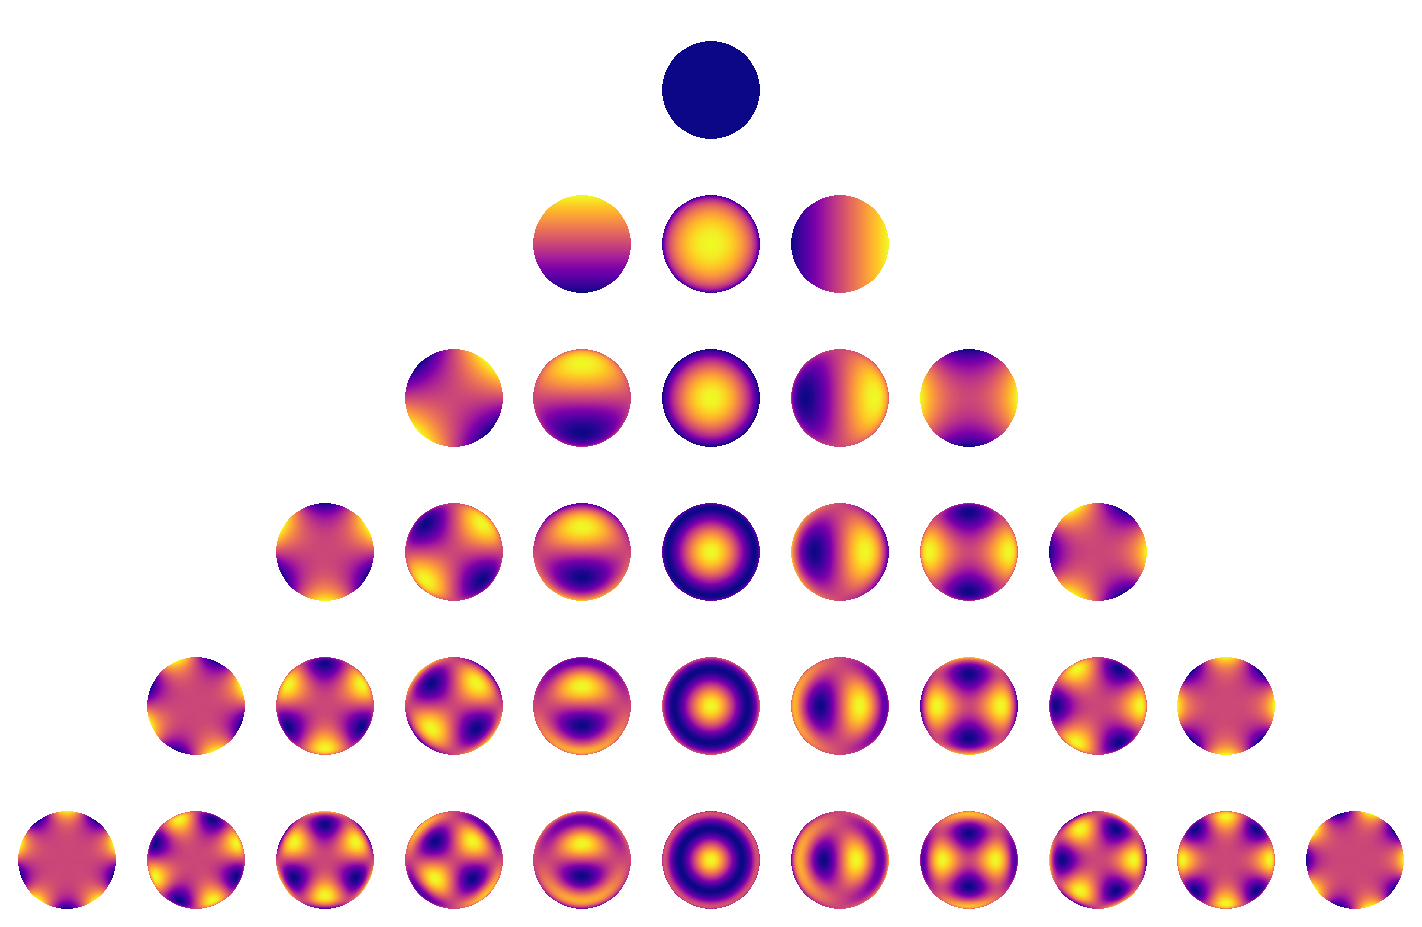
\includegraphics[width=\linewidth]{figures/ylms.pdf}
    \caption{\label{fig:ylms}
             \animation{ylms}
             The real spherical harmonics up to degree $l = 5$ computed from
             Equation~(\ref{eq:ylmtp}). In these plots, the $x$-axis points
             to the right,
             the $y$-axis points up, and the $z$-axis points
             out of the page.
             \python{ylms}Click on the link on the right to view an
             animated version.}
    \end{centering}
\end{figure}
%
Re-writing Equation~(\ref{eq:ylmtp}) in terms of $\x$, $\y$, and $\z$ leads
to expressions that are simply polynomials of these variables, a fact we will
heavily exploit below when computing their integrals.
We derive the polynomimal representation of the spherical harmonics
in Appendix~\ref{app:spharm}. The spherical harmonics up to
degree $l = 5$ are shown in Figure~\ref{fig:ylms}.

% ------------------------------------------------------------------------------
\subsection{Surface map vectors}
\label{sec:vectors}
% ------------------------------------------------------------------------------

Any physical surface map of a celestial body can be expanded in terms of
the real spherical harmonics defined in the previous section. For
convenience, in this paper we represent a surface map as a
vector $\bvec{y}$ of spherical harmonic
coefficients such that the specific intensity at the point
$(\x, \y)$ may be written
%
\begin{align}
    \label{eq:I}
    I(\x, \y) = \ybasis^\mathsf{T} (\x, \y) \, \bvec{y}
    \quad,
\end{align}
%
where $\ybasis$ is the \emph{spherical harmonic basis},
arranged in increasing degree and order:
%
\begin{align}
    \label{eq:by}
    \ybasis =
    \begin{pmatrix}
        Y_{0, 0} &
        Y_{1, -1} & Y_{1, 0} & Y_{1, 1} &
        Y_{2, -2} & Y_{2, -1} & Y_{2, 0} & Y_{2, 1} & Y_{2, 2} &
        \cdot\cdot\cdot
    \end{pmatrix}^\mathsf{T}
    \quad,
\end{align}
%
where $Y_{l, m} = Y_{l, m}(\x, \y)$ are given by \eq{ylmxy}.
For reference, in this basis the coefficient of the spherical harmonic
$Y_{l, m}$ is located at the index
%
\begin{align}
    \label{eq:n}
    n = l^2 + l + m
\end{align}
%
of the vector $\bvec{y}$. Conversely, the coefficient at index $n$
of $\bvec{y}$ corresponds
to the spherical harmonic of degree and order given by
%
\begin{align}
    \label{eq:lm}
    l &= \floor*{\sqrt{n}} \nonumber \\
    m &= n - \floor*{\sqrt{n}}^2 - \floor*{\sqrt{n}}
    \quad.
\end{align}
%

% ------------------------------------------------------------------------------
\subsection{Change of basis}
\label{sec:basis}
% ------------------------------------------------------------------------------

In order to compute the occultation light curve for a body with a given surface
map $\bvec{y}$, it is convenient to first find its polynomial representation
$\bvec{p}$, which we express as a vector of coefficients in the
\emph{polynomial basis} $\pbasis$:
%
\begin{align}
    \label{eq:bp}
    \pbasisn &=
    \begin{dcases}
        \x^\frac{\mu}{2} \y^\frac{\nu}{2} & \qquad \nu \, \mathrm{even}
        \\
        \x^\frac{\mu-1}{2} \y^\frac{\nu-1}{2} \z & \qquad \nu \, \mathrm{odd}
    \end{dcases}
    \nonumber\\[0.5em]
    \pbasis &=
    \begin{pmatrix}
        1 &
        \x & \z & \y &
        \x^2 & \x\z & \x\y & \y\z & \y^2 &
        \cdot\cdot\cdot
    \end{pmatrix}^\mathsf{T}
    \quad,
    \mathematica{A1}
\end{align}
%
where
%
\begin{align}
    \label{eq:munu}
    \mu &= l - m \nonumber \\
    \nu &= l + m
    \quad
\end{align}
%
with $l$ and $m$ given by \eq{lm}.
%
%
To find $\bvec{p}$ given $\bvec{y}$, we
introduce the change of basis matrix $\AOne$,
which transforms
a vector in the spherical harmonic basis $\ybasis$ to the
polynomial basis $\pbasis$:
%
\begin{align}
    \bvec{p} = \AOne \, \bvec{y}
\end{align}
%
The columns of $\AOne$ are simply the polynomial vectors
corresponding to each of the spherical harmonics in \eq{by}; see
Appendix~\ref{app:basis} for details.
%
As before, the specific intensity at the point $(\x, \y)$
may be computed as
%
\begin{align}
    I(\x, \y) &= \pbasis^\mathsf{T} \bvec{p} \nonumber \\
              &= \pbasis^\mathsf{T} \AOne \, \bvec{y}
    \quad.
\end{align}

As we will see in the next section, integrating the surface map over the disk of
the body is easier if we apply one final transformation to our input vector,
rotating it into what we will refer to as the \emph{Green's basis}, $\gbasis$:
%
\begingroup\makeatletter\def\f@size{10}\check@mathfonts
\def\maketag@@@#1{\hbox{\m@th\normalsize#1}}%
\begin{align}
    \label{eq:bg}
    \gbasisn &=
    \begin{dcases}
        %
        \frac{\mu+2}{2}\x^\frac{\mu}{2} \y^\frac{\nu}{2}
            & \qquad \nu \, \mathrm{even}
        \\[1em]
        %
        \z
            & \qquad l = 1, \, m = 0
        \\[1em]
        %
        3\x^{l-2}\y\z
            & \qquad \nu \, \mathrm{odd}, \,
                     \mu = 1, \,
                     l \, \mathrm{even}
        \\[1em]
        %
        \z
        \bigg(
         -\x^{l-3} + \x^{l-1} + 4\x^{l-3}\y^2
        \bigg)
         & \qquad \nu \, \mathrm{odd}, \,
                  \mu = 1, \,
                  l \, \mathrm{odd}
        \\[1em]
        %
        \z
        \bigg(
            \frac{\mu-3}{2} \x^\frac{\mu-5}{2} \y^\frac{\nu-1}{2}
            -
            \frac{\mu-3}{2} \x^\frac{\mu-5}{2} \y^\frac{\nu+3}{2}
            -
            \frac{\mu+3}{2} \x^\frac{\mu-1}{2} \y^\frac{\nu-1}{2}
        \bigg)
            & \qquad \mathrm{otherwise}
    \end{dcases}
    \nonumber\\[1.5em]
    \gbasis &=
    \begin{pmatrix}
        1 &
        2\x & \z & \y &
        3\x^2 & -3\x\z & 2\x\y & 3\y\z & \y^2 &
        \cdot\cdot\cdot
    \end{pmatrix}^\mathsf{T}
    \quad,
    \mathematica{A2}
\end{align}
\endgroup
%
where the values of $l$, $m$, $\mu$, and $\nu$ are given by
Equations~(\ref{eq:lm}) and (\ref{eq:munu}). Given
a polynomial vector $\bvec{p}$, the corresponding vector in
the Green's basis, $\bvec{g}$, can be found by performing another
change of basis operation:
%
\begin{align}
    \bvec{g} = \bvec{\ATwo} \, \bvec{p}
\end{align}
%
where the columns of the matrix $\ATwo$ are the Green's vectors
corresponding to each of the polynomial terms in \eq{bp};
see Appendix~\ref{app:basis} for details.

Note that we may also transform directly from the spherical harmonic basis
to the Green's basis:
%
\begin{align}
    \bvec{g} &= \ATwo \, \AOne \, \bvec{y} \nonumber \\
             &= \bvec{A} \, \bvec{y}
\end{align}
%
where
%
\begin{align}
    \label{eq:A}
    \bvec{A} \equiv \ATwo \, \AOne
\end{align}
%
is the full change of basis matrix.
%
For completeness,
we again note that the specific intensity at a point on a map
described by the spherical harmonic vector $\bvec{y}$ may be written
%
\begin{align}
    \label{eq:fluxpoint}
    I(\x, \y) &= \gbasis^\mathsf{T}(\x, \y) \bvec{g} \nonumber \\
              &= \gbasis^\mathsf{T}(\x, \y) \bvec{A} \, \bvec{y}
    \quad.
\end{align}
%

% ------------------------------------------------------------------------------
\subsection{Rotation of surface maps}
\label{sec:rotation}
% ------------------------------------------------------------------------------

Defining a map as a vector of spherical harmonic coefficients makes it
straightforward to compute the projection of the map under arbitrary rotations
of the body via a rotation matrix $\bvec{R}$:
%
\begin{align}
    \label{eq:rotation}
    \bvec{y'} = \bvec{R} \, \bvec{y}
\end{align}
%
where $\bvec{y'}$ are the spherical harmonic coefficients of the rotated map.
In Appendix~\ref{app:rotation} we derive expressions for $\bvec{R}$ in terms
of the Euler angles $\alpha$, $\beta$, and $\gamma$, as well as in terms of
an angle $\theta$ and an arbitrary axis of rotation $\bvec{u}$. Follow the link
next to Figure~\ref{fig:ylms} to view an animation of the spherical harmonics
rotating about the $y$-axis, computed from \eq{rotation}.


% ==============================================================================
% ------------------------------------------------------------------------------
% ------------------------------------------------------------------------------
\section{Computing light curves}
\label{sec:lightcurves}
% ------------------------------------------------------------------------------
% ------------------------------------------------------------------------------
% ==============================================================================

% ------------------------------------------------------------------------------
\subsection{Rotational phase curves}
\label{sec:phasecurves}
% ------------------------------------------------------------------------------

Consider a body of unit radius centered at the origin, with a surface map
given by the spherical harmonic vector $\bvec{y}$ viewed at an orientation
specified by the rotation matrix $\bvec{R}$, such that
the specific intensity at a point $(\x, \y)$ on the surface is
%
\begin{align}
    I(\x, \y) &= \ybasis^\mathsf{T} (\x, \y) \bvec{R} \, \bvec{y}
    \nonumber \\
              &= \pbasis^\mathsf{T} (\x, \y) \AOne \, \bvec{R} \, \bvec{y}
    \quad
\end{align}
%
where $\pbasis$ is the polynomial basis and $\AOne$ is the corresponding
change-of-basis matrix (\S\ref{sec:basis}).
The total flux radiated
in the direction of the observer is obtained by integrating the specific
intensity over a region $S$ of the projected disk of the body:
%
\begin{align}
    \label{eq:phaseint}
    F &=
    \oiint I(\x, \y) \, \dd S
    \nonumber \\
    &=
    \oiint \pbasis^\mathsf{T} (\x, \y) \AOne \, \bvec{R} \, \bvec{y} \, \dd S
    \nonumber \\
    &=
    \bvec{r}^\mathsf{T} \AOne \, \bvec{R} \, \bvec{y}
    \quad,
\end{align}
%
where $\bvec{r}$ is a column vector whose $n^\mathrm{th}$ component is given by
%
\begin{align}
    \label{eq:rn}
    r_n &\equiv
      \oiint \pbasisn (\x, \y)  \, \dd S
    \quad.
\end{align}
%
When the entire disk of the body is visible (i.e., when no occultation is
occurring), this may be written
%
\begin{align}
    r_n &=
              \int_{-1}^{1}
              \int_{-\sqrt{1-\x^2}}^{\sqrt{1+\x^2}}
              \tilde{p}_n (\x, \y)
              \,
              \dd \y \, \dd \x
        \nonumber \\[1em]
        &=
        \begin{dcases}
            \frac{
                    \Gamma\left(\frac{\mu}{4} + \frac{1}{2}\right)
                    \Gamma\left(\frac{\nu}{4} + \frac{1}{2}\right)
                }{
                    \Gamma\left(\frac{\mu + \nu}{4} + 2\right)
                }
            & \qquad \frac{\mu}{2} \, \mathrm{even}, \, \frac{\nu}{2} \, \mathrm{even}
            %
            \\[1em]
            %
            \frac{\sqrt{\pi}}{2}
            \frac{
                    \Gamma\left(\frac{\mu}{4} + \frac{1}{4}\right)
                    \Gamma\left(\frac{\nu}{4} + \frac{1}{4}\right)
                }{
                    \Gamma\left(\frac{\mu + \nu}{4} + 2\right)
                }
            & \qquad \frac{\mu-1}{2} \, \mathrm{even}, \, \frac{\nu-1}{2} \, \mathrm{even}
            %
            \\[1em]
            %
            0
            & \qquad \mathrm{otherwise.}
        \end{dcases}
    \mathematica{rn}
\end{align}
%
where $\Gamma(\bigdot)$ is the gamma function.
%
\eq{phaseint} may be used to analyticly compute the rotational (thermal) phase curve of a body
with an arbitrary surface map. Since $\bvec{r}$ and $\bvec{A_1}$ are independent
of the map coefficients or its orientation, these may be pre-computed for
computational efficiency.

We note, finally, that a form of this solution was very recently found by \citet{Haggard2018};
a special case of their equations for phase curves in reflected light yields
analytic expressions for thermal phase curves of spherical harmonics.

% HACK
\pagebreak
% HACK

% ------------------------------------------------------------------------------
\subsection{Occultation light curves}
\label{sec:occultationflux}
% ------------------------------------------------------------------------------

As we showed earlier, the specific intensity
at a point $(\x, \y)$ on the surface of a body described by the map $\bvec{y}$
and the rotation matrix $\vec{R}$ may also be written as
%
\begin{align}
    I(\x, \y) &= \ybasis^\mathsf{T} (\x, \y) \bvec{R} \, \bvec{y}
    \nonumber \\
              &= \gbasis^\mathsf{T} (\x, \y) \bvec{A} \, \bvec{R} \, \bvec{y}
    \quad,
\end{align}
%
where $\gbasis$ is the Green's basis and $\bvec{A}$ is the full change of basis
matrix (\S\ref{sec:basis}).
As before, the total flux radiated
in the direction of the observer is obtained by integrating the specific
intensity over a region $S$ of the projected disk of the body:
%
\begin{align}
    \label{eq:occint}
    F &=
    \oiint I(\x, \y) \, \dd S
    \nonumber \\
    &=
    \oiint \gbasis^\mathsf{T} (\x, \y) \, \dd S \, \bvec{A} \, \bvec{R} \, \bvec{y}\quad.
\end{align}
%
This time, suppose the body is
occulted by another body of radius $r$ centered at the point $(x_o, y_o)$,
so that the surface $S$ over which the integral is taken
is a function of $r$, $x_o$, and $y_o$.
In general, the integral in \eq{occint} is
difficult (and often impossible) to compute directly.
%
One way to simplify the problem is to first perform a rotation through an angle
%
\begin{align}
    \label{eq:zrot}
    \omega = \frac{\pi}{2} - \mathrm{arctan2}(y_o, x_o)
\end{align}
%
about the $z$-axis ($\bvec{u} = \left[0, 0, 1\right]$)
so that the occultor lies along the
$+y$-axis, with its center located a distance $b = \sqrt{x_o^2 + y_o^2}$
from the origin (see Figure~\ref{fig:geometry}).
%
In this rotated frame, the limits of integration (the two points of intersection
between the occultor and the occulted body, should they exist)
are symmetric about the $y$-axis.
If we define $\phi \in [-\nicefrac{\pi}{2}, \, \nicefrac{\pi}{2}]$
as the angular position of the right hand side intersection point
relative to the occultor center, measured counter-clockwise
from the $+x$ direction, the arc of the occultor that overlaps the occulted
body extends from $\pi - \phi$ to $2\pi + \phi$ (see the Figure).
Similarly, defining $\lambda \in [-\nicefrac{\pi}{2}, \, \nicefrac{\pi}{2}]$
as the angular position of the same point relative to the origin, the
arc of the portion of the occulted body that is visible during the occultation
extends from $\pi - \lambda$ to $2\pi + \lambda$ (see the Figure).
%
For future reference, it can be shown that
%
\begin{align}
    \label{eq:phi}
    \phi &=
    \begin{dcases}
        \arcsin\left({\frac{1 - r^2 - b^2}{2br}}\right)
                                                & \qquad |1 - r| < b < 1 + r \\
        \frac{\pi}{2}                           & \qquad b \le 1 - r
    \end{dcases}
    \mathematica{philam} \\
\intertext{and}
    \label{eq:lambda}
    \lambda &=
    \begin{dcases}
        \arcsin\left(\frac{1 - r^2 + b^2}{2b}\right)
                                                & \qquad |1 - r| < b < 1 + r \\
        \frac{\pi}{2}                           & \qquad b \le 1 - r
        \quad,
    \end{dcases}
    \mathematica{philam}
\end{align}
%
The case $b \le 1 - r$ corresponds to an occultation during which the occultor
is fully within the planet disk, so no points of intersection exist.
In this case,
we define $\phi$ such that the arc from $\pi - \phi$ to $2\pi + \phi$ spans the
entire circumference of the occultor, and $\lambda$ such that the arc
from $\pi - \lambda$ to $2\pi + \lambda$ spans the
entire circumference of the occulted body.
Note that if $b \ge 1 + r$, no occultation occurs and the flux may
be computed as in \S\ref{sec:phasecurves}, while
if $b \le r - 1$, the entire disk of the body is occulted and the total flux
is zero.

The second trick we employ to solve \eq{sn} is to use
Green's theorem to express the surface integral of $\gbasis_n$ as the
line integral of a vector function $\bvec{G}_n$ along the boundary of
the same surface \citep{Pal2012}. Defining the ``solution'' column vector
%
\begin{align}
    \label{eq:sndef}
    \bvec{s}^\mathsf{T} &\equiv
      \oiint \gbasis^\mathsf{T} (\x, \y)  \, \dd S
    \quad,
\end{align}
%
we may write its $n^\mathrm{th}$ component as
%
\begin{align}
    \label{eq:greens}
    s_n &=
    \oiint \gbasisn (\x, \y) \, \dd S
    =
    \oint \bvec{G}_n (\x, \y) \cdot \dd \bvec{r}
    \quad,
\end{align}
%
where $\bvec{G}_n (\x, \y) = {G_n}_x (\x, \y) \, \xhat + {G_n}_y (\x, \y) \, \yhat$ is
chosen such that
%
\begin{align}
    \label{eq:DGg}
    \bvec{D} \wedge \bvec{G}_n = \gbasisn(\x, \y)
    \quad.
\end{align}
%
The operation $\bvec{D} \wedge \bvec{G}_n$ denotes the
\emph{exterior derivative} of $\bvec{G}_n$. In two-dimensional Cartesian
coordinates, it is given by
%
\begin{align}
    \label{eq:extderiv}
    \bvec{D} \wedge \bvec{G}_n &\equiv \frac{\dd {G_n}_y}{\dd \x}
                                   - \frac{\dd {G_n}_x}{\dd \y} \quad.
\end{align}
%
%
Thus, in order to compute $s_n$ in \eq{greens}, we must (1) apply a rotation
to our map $\bvec{y}$ to align the occultor with the $+y$-axis;
(2) find a vector function
$\bvec{G}_n$ whose exterior derivative is the $n^\mathrm{th}$ component of the
vector basis $\gbasis$ (Equation~\ref{eq:bg}); and
(3) integrate it along the boundary of the visible portion of the occulted
body's surface. In general, for an occultation involving two bodies,
this boundary consists of two arcs: a segment of the circle bounding the
occultor (thick red curve in Figure~\ref{fig:geometry}),
and a segment of the circle bounding the occulted body (thick black curve
in Figure~\ref{fig:geometry}).
%
If we happen to know $\bvec{G}_n$, the integral in \eq{greens} is just
%
\begin{align}
    \label{eq:sn}
    s_n &= \mathcal{Q}(\bvec{G}_n) - \mathcal{P}(\bvec{G}_n)
    \quad,
\end{align}
%
where, as in \citet{Pal2012}, we define the \emph{primitive integrals}
%
\begin{align}
    \label{eq:primitiveP}
    \mathcal{P}(\bvec{G}_n) &=
    \int\displaylimits_{\pi-\phi}^{2\pi + \phi}
        \big[ {G_n}_y(r c_\varphi, b + r s_\varphi) c_\varphi -
              {G_n}_x(r c_\varphi, b + r s_\varphi) s_\varphi \big] r \dd \varphi
    \\
    %
\intertext{and}
    %
    \label{eq:primitiveQ}
    \mathcal{Q}(\bvec{G}_n) &=
    \int\displaylimits_{\pi-\lambda}^{2\pi + \lambda}
        \big[ {G_n}_y(c_\varphi, s_\varphi) c_\varphi -
              {G_n}_x(c_\varphi, s_\varphi) s_\varphi \big] \dd \varphi
    \quad,
\end{align}
%
%
where, as before,
$c_\varphi \equiv \cos \varphi$
and
$s_\varphi \equiv \sin \varphi$
and we used the fact that along the arc of a circle,
%
\begin{align}
    \label{eq:dr}
    \dd \bvec{r} &= -r s_\varphi \, \dd \varphi \, \xhat +
                     r c_\varphi \, \dd \varphi \, \yhat
    \quad.
\end{align}
%
In Equations~(\ref{eq:primitiveP}) and (\ref{eq:primitiveQ}), $\mathcal{P}(\bvec{G}_n)$
is the line integral along the arc of the occultor
and $\mathcal{Q}(\bvec{G}_n)$ is the line integral along the arc of the occulted
body.

%
%
\begin{figure}[p!]
    \begin{centering}
    \includegraphics[width=\linewidth]{figures/geometry.pdf}
    \caption{\label{fig:geometry}
             \python{geometry}
             Geometry of the occultation problem.
             The occulted body is centered
             at the origin and has unit radius, while the occultor
             is centered at $(x_o, y_o)$ and has radius $r$. We first rotate
             the two bodies about the origin through an angle
             $\theta = \nicefrac{\pi}{2} - \mathrm{arctan2}(y_o, x_o)$
             so the problem is symmetric about the $y$-axis. In this frame,
             the occultor is located at $(0, b)$, where
             $b = \sqrt{x_o^2 + y_o^2}$ is the impact parameter.
             The arc of the occultor
             that overlaps the occulted body (thick red curve) now extends from
             $\pi - \phi$ to $2\pi + \phi$, measured from the center of the
             occultor.
             The arc of the occulted body that is visible during
             the occultation (thick black curve) extends from
             $\pi - \lambda$ to $2\pi + \lambda$, measured from the origin.
             These are the curves along which the primitive integrals
             (Equations~\ref{eq:primitiveP} and \ref{eq:primitiveQ}) are evaluated.
             The angles $\phi$ and $\lambda$ are given by
             Equations~(\ref{eq:phi}) and (\ref{eq:lambda})
             and extend from $-\nicefrac{\pi}{2}$ to $\nicefrac{\pi}{2}$. When
             the occultor is completely within the disk of the occulted body,
             we define $\phi = \lambda = \nicefrac{\pi}{2}$.
             }
    \end{centering}
\end{figure}
%
%

As cumbersome as the Green's basis (Equation~\ref{eq:bg}) may appear, the reason
we introduced it is that its anti-exterior derivatives are conveniently simple.
It can be easily shown that one possible solution to \eq{DGg} is
%
\begin{align}
    \label{eq:Gn}
    \bvec{G}_n (\x, \y) &=
    \begin{dcases}
        %
        \x^{\frac{\mu + 2}{2}}
        \y^{\frac{\nu}{2}}
        \,\yhat
            & \qquad \nu \, \mathrm{even}
        \\[1em]
        %
        \frac{1-z^3}{3(1-z^2)}(-\y \, \xhat + \x \, \yhat)
            & \qquad l = 1, \, m = 0
        \\[1em]
        %
        \x^{l-2}
        \z^3
        \,\xhat
            & \qquad \nu \, \mathrm{odd}, \,
                     \mu = 1, \,
                     l \, \mathrm{even}
        \\[1em]
        %
        \x^{l-3}
        \y
        \z^3
        \,\xhat
         & \qquad \nu \, \mathrm{odd}, \,
                  \mu = 1, \,
                  l \, \mathrm{odd}
        \\[1em]
        %
        \x^{\frac{\mu-3}{2}}
        \y^{\frac{\nu-1}{2}}
        \z^3
        \,\yhat
            & \qquad \mathrm{otherwise,}
    \end{dcases}
    \mathematica{G}
\end{align}
%
where $l$ and $m$ are given by \eq{lm} and $\mu$ and $\nu$ are given by
\eq{munu}. Solving the occultation problem is therefore a matter of
evaluating the primitive integrals of $\bvec{G}_n$
(Equations~\ref{eq:primitiveP} and \ref{eq:primitiveQ}).
The solutions are in general tedious, but
they are all analytic, involving sines, cosines, and complete elliptic integrals.
In Appendix~\ref{app:solutionvector} we derive recurrence
relations to quickly compute these. We note, in particular, that the
solutions all involve complete elliptic integrals of the \emph{same} argument,
so that the elliptic integrals need only be evaluated once for a map
of arbitrary degree, greatly improving the evaluation speed and the
scalability of the problem to high order.

% ------------------------------------------------------------------------------
\subsection{Summary}
\label{sec:summary}
% ------------------------------------------------------------------------------

Here we briefly summarize how to analytically compute the flux during
an occultation of a body whose specific intensity profile is described
by a sum of spherical harmonics. Given a body of unit radius with a
surface map described by the vector of spherical harmonic coefficients
$\mathbf{y}$ (Equation~\ref{eq:by}), occulted by another body of radius $r$
centered at the point $(x_o, y_o)$, we must:
%
\begin{enumerate}
    \item Compute the rotation matrix $\bvec{R}$ to rotate the map to the correct
          viewing orientation, which may be
          specified by the Euler angles $\alpha$, $\beta$, and $\gamma$
          (Appendix~\ref{app:euler}) or by an axis $\bvec{u}$ and an angle $\theta$
          (Appendix~\ref{app:axisangle}).
    \item Compute the rotation matrix $\bvec{R'}$ to rotate the map
          by an angle $\omega$ about the $+z$-axis
          (Equation~\ref{eq:zrot}) so the center of the occultor is a
          distance $b = \sqrt{x_o^2 + y_o^2}$ along the $+y$-axis
          from the center of the occulted body.
    \item Compute the change-of-basis matrix $\bvec{A}$ (\S\ref{sec:basis}) to
          convert our vector of spherical harmonic coefficients to a vector
          of polynomial coefficients in the Green's basis
          (Equation~\ref{eq:bg}). Since $\bvec{A}$ is the same for all
          occultations, this matrix may be pre-computed to improve
          computational speed.
    \item Compute the solution vector $\bvec{s}$ (Equation~\ref{eq:sn}), with
          $\mathcal{P}(\bvec{G}_n)$ and $\mathcal{Q}(\bvec{G}_n)$ given by
          Equations~(\ref{eq:PGnI}) and (\ref{eq:QGnI}) in the Appendix.
          Note that $s_2$ is special and must be computed separately
          (Equation~\ref{eq:s2}).
\end{enumerate}
%
Given these quantities, the total flux during an occultation is then just
%
\begin{equation}
    \label{eq:starry}
    \boxed{
        %\large
        F = \bvec{s}^{\boldsymbol{\mathsf{T}}} \bvec{A} \, \bvec{R'} \, \bvec{R} \, \bvec{y}
        }
    \quad.
\end{equation}   % This is about the nerdiest pun I've ever seen
% (with the exception "It's amazing that 230-220 x 1/2 = 5!")


% ==============================================================================
% ------------------------------------------------------------------------------
% ------------------------------------------------------------------------------
%\pagebreak
\section{The \textbf{STARRY} code package}
\label{sec:starrycode}
% ------------------------------------------------------------------------------
% ------------------------------------------------------------------------------
% ==============================================================================

The \starry code package provides code to analytically
compute light curves for celestial bodies using the formalism developed
in this paper. \starry is coded entirely in \cpp for speed and wrapped
in \Python using \pybind \citep{pybind11} for quick and easy
light curve calculations. The
code may be installed by running the following in a terminal:
%
\begin{lstlisting}[language=bash]
git clone https://github.com/rodluger/starry.git
cd starry
python setup.py develop
\end{lstlisting}
%
There are two primary ways of interfacing with \starry: via the surface
map class \starryMap and via the celestial body system class
\starrySystem. The former gives users the most flexibility to
create and manipulate surface maps and compute their fluxes for a variety
of applications, while the latter provides a quick and easy (but limited)
way to generate light curves for exoplanet systems. Let us
discuss the map class first.

% ------------------------------------------------------------------------------
\subsection{Creating a map}
\label{sec:starrymap}
% ------------------------------------------------------------------------------

To begin using \starry, execute the following in a \Python environment:
%
\begin{lstlisting}[language=Python]
from starry import Map
\end{lstlisting}
%
A \starry \Map is a vector of spherical harmonic coefficients, indexed by
increasing degree and order, as in \eq{by}. We can create a map of
spherical harmonics up to degree $l_\mathrm{max} = 5$ by typing
%
\begin{lstlisting}[language=Python,firstnumber=last]
map = Map(5)
\end{lstlisting}
%
By default, all coefficients are set to zero.
Say our surface map is given by the function
%
\begin{align}
    \label{eq:ylm_code_example}
    I(\x, \y) &= -2 Y_{5,-3}(\x, \y) + 2 Y_{5,0}(\x, \y) + Y_{5,4}(\x, \y)
    \quad.
\end{align}
%
To instantiate this map, we set the corresponding coefficients in \map:
%
\begin{lstlisting}[language=Python,firstnumber=last]
map[5, -3] = -2
map[5, 0] = 2
map[5, 4] = 1
\end{lstlisting}
%
Printing the map to screen yields
%
\begin{lstlisting}[language=Python,numbers=none]
<STARRY Map: -2 Y_{5,-3} + 2 Y_{5,0} + Y_{5,4}>
\end{lstlisting}
%
Users can also directly access the spherical harmonic vector $\bvec{y}$,
polynomial vector $\bvec{p}$, and Green's polynomial vector $\bvec{g}$
via the attributes \starryMapy, \starryMapp, and \starryMapg, respectively.
%
%\begin{lstlisting}[language=Python,numbers=none]
%# map.y
%[0, 0, 0, 0, 0, 0, 0, 0, 0, 0, 0, 0, 0, 0, 0, 0, 0, 0, 0,
% 0, 0, 0, 0, 0, 0, 0, 0, -2, 0, 0, 2, 0, 0, 0, 1, 0]
%
%# map.p
%[0, 0, 1.87, 0, 0, 0, 0, 0, 0, 0, -13.10, -23.48, 0, 0,
% -13.10, 7.83, 0, 0, 0, 0, 0, 0, 0, 0, 0, 0, 16.81, 26.42,
% 0, 0, 17.02, 17.61, 0, 0, 16.81, -8.81]
%
%# map.g
%[0, 0, 0, 0, 0, 0, 0, 0, 0, 0, 3.73, -7.83, 0, 0, 1.86,
% 7.83, 0, 0, 0, 0, 0, 0, 0, 0, 0, 0, -5.59, 5.28, 0, 0,
% -16.81, 5.87, 0, 0, -16.75, -8.81])
%\end{lstlisting}
%
Once a map is instantiated, users may quickly visualize it by calling
%
\begin{lstlisting}[language=Python,firstnumber=last]
map.show()
\end{lstlisting}
%
or
%
\begin{lstlisting}[language=Python,firstnumber=last]
map.animate(axis=axis)
\end{lstlisting}
%
where \textsf{axis} defines the axis of rotation for the animation.
Rotation of this map about $\yhat$ yields\python{smiley}
%
\begin{center}
    \includegraphics[width=0.85\linewidth]{figures/smiley.pdf}
\end{center}
%

Alternatively, users may provide the path to an image file of the
surface map on a rectangular latitude-longitude grid or a ring-ordered
\textsf{Healpix}\footnote{\url{http://healpix.sf.net}} map array:
%
\begin{lstlisting}[language=Python,firstnumber=last]
map.load_image("/path/to/image.jpg")
\end{lstlisting}
%
or
%
\begin{lstlisting}[language=Python,firstnumber=last]
map.load_healpix(array)
\end{lstlisting}
%
In both cases, \starry uses the \textsf{map2alm()} function
of the \textsf{healpy} package to find the expansion of the map in
terms of spherical harmonics. Keep in mind that if the image contains very dark
pixels (with \textsf{RGB} values close to zero), its spherical harmonic
expansion may lead to regions with \emph{negative} specific intensity, which
is of course unphysical.

In Figure~\ref{fig:earth} we show a
simplified two-color map of the cloudless Earth and its corresponding
\starry instance for
$l_\mathrm{max} = 10$, rotated successively about $\yhat$.
%
\begin{figure}[ht!]
    \begin{centering}
    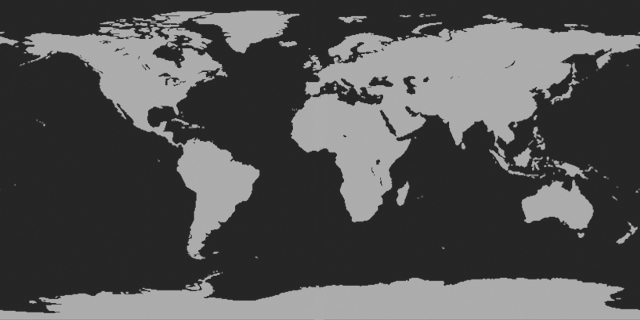
\includegraphics[width=0.8\linewidth]{figures/earth.jpg}
    \\[1em]
    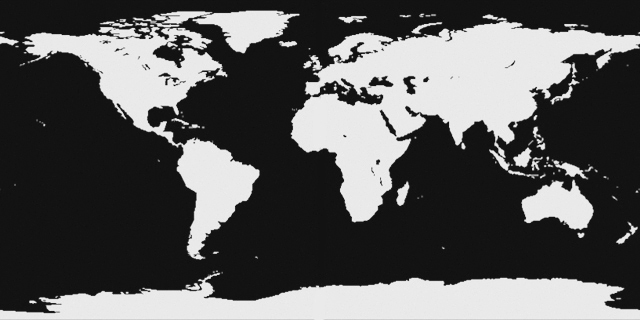
\includegraphics[width=0.85\linewidth]{figures/earth.pdf}
    \caption{\label{fig:earth}
             \python{earth}
             A simplified two-color map of the cloudless Earth (top) and the
             corresponding tenth-degree spherical harmonic expansion,
             rotated about $\yhat$ (bottom).}
    \end{centering}
\end{figure}
%

% ------------------------------------------------------------------------------
\subsection{Computing rotational phase curves}
\label{sec:starryphasecurves}
% ------------------------------------------------------------------------------
%
\begin{figure}[p!]
    \begin{centering}
    \includegraphics[width=\linewidth]{figures/ylmphasecurves.pdf}
    \\[1em]
    \includegraphics[width=\linewidth]{figures/ylmlightcurves.pdf}
    \caption{\label{fig:ylmlightcurves}
             \python{ylmphasecurves}
             \emph{Top:} Phase curves for the first several spherical
             harmonics with order $m \ge 0$ rotated about the $x$-axis
             (blue) and about the $y$-axis (orange).
             Odd harmonics with $l > 1$ and harmonics with $m < 0$ are
             \python{ylmlightcurves}
             in the phase curve null space \citep{CowanFuentesHaggard2013}.
             \emph{Bottom:} Occultation light curves for the same
             set of spherical harmonics. An occultor of radius $r=0.3$
             transits the body along the $+\x$ direction at $y_o = 0.25$
             (blue) and $y_o = 0.75$ (orange). }
    \end{centering}
\end{figure}
%
Once a map is instantiated, it is easy to compute its rotational
phase curve, \textsf{F}:
%
\begin{lstlisting}[language=Python,firstnumber=last]
F = map.flux(axis=axis, theta=theta)
\end{lstlisting}
%
where \textsf{axis} is the axis of rotation and \textsf{theta} is an array of
angles (in radians) for which to compute the flux. Note that rotations performed
by \flux are not cumulative; instead, all angles should be specified
relative to the original, unrotated map frame.
%
In the top panel of Figure~\ref{fig:ylmlightcurves} we plot rotational phase curves
for all spherical harmonics
up to $l_\mathrm{max} = 6$ for rotation about $\xhat$ (blue curves) and $\yhat$
(orange curves). The small dots correspond to phase curves computed by numerical
evaluation of the flux on an adaptive radial mesh (see \S\ref{sec:starrybenchmarks}).
As discussed by \citet{CowanFuentesHaggard2013}, harmonics with
odd $l > 1$ and those with $m < 0$ (not plotted) are in the null space and
therefore do not exhibit rotational phase variations.

%

As a second example, we can compute the rotational phase curve of the simplified Earth model
(Figure~\ref{fig:earth}) for rotation about $\yhat$ (its actual spin axis)
by executing
%
\begin{lstlisting}[language=Python,firstnumber=last]
theta = np.linspace(0, 360, 100)
F = map.flux(axis=[0, 1, 0], theta=theta)
\end{lstlisting}
%
The variable $\textsf{F}$ is
an array of flux values computed from \eq{phaseint}; we plot this in
Figure~\ref{fig:earthphasecurve}, alongside the rotational phase curves due to each of
the seven individual continents.
%
\begin{figure}[ht!]
    \begin{centering}
    \includegraphics[width=\linewidth]{figures/earthphasecurve.pdf}
    \caption{\label{fig:earthphasecurve}
             \python{earthphasecurve}
             Phase curve for the Earth rotating about its axis, computed
             from the $l_\mathrm{max} = 10$ expansion from
             Figure~\ref{fig:earth}. The full rotational phase curve is shown in black,
             and the flux due to each of the seven continents is shown as
             the colored curves (see legend). The black dots correspond to the
             numerical solution.}
    \end{centering}
\end{figure}
%

% ------------------------------------------------------------------------------
\subsection{Computing occultation light curves}
\label{sec:starryoccultation}
% ------------------------------------------------------------------------------

Occultation light curves are similarly easy to compute:
%
\begin{lstlisting}[language=Python,firstnumber=last]
F = map.flux(axis=axis, theta=theta, xo=xo, yo=yo, ro=ro)
\end{lstlisting}
%
where \textsf{axis} and \textsf{theta} are the same as above, and
\textsf{xo}, \textsf{yo}, and \textsf{ro} are the occultor parameters
($\x$ position, $\y$ position, and radius, all in units of the
occulted body's radius), which may be either scalars
or arrays.

%

In the bottom panel of Figure~\ref{fig:ylmlightcurves} we plot
occultation light curves for the spherical harmonics with $m \ge 0$
up to $l_\mathrm{max} = 6$. The occultor has radius $r = 0.3$ and
moves at a constant speed along the $\x$ direction at $y_o = 0.25$
(blue curves) and $y_o = 0.75$ (orange curves). The light curve of
any body undergoing such an occultation can be expressed as a weighted
sum of these light curves. Note that because the value of individual
spherical harmonics can be negative, an increase in the flux is visible
at certain points during the occultation; however, this would of course not
occur for any physical map constructed from a linear combination of
the spherical harmonics. Note also that unlike in the case of rotational phase curves,
there is no null space for occultations, as all spherical harmonics (including
those with $m < 0$, which are not shown) produce a flux signal during
occultation. As before, the numerical solutions are shown as the small dots.

%
\begin{figure}[ht!]
    \begin{centering}
    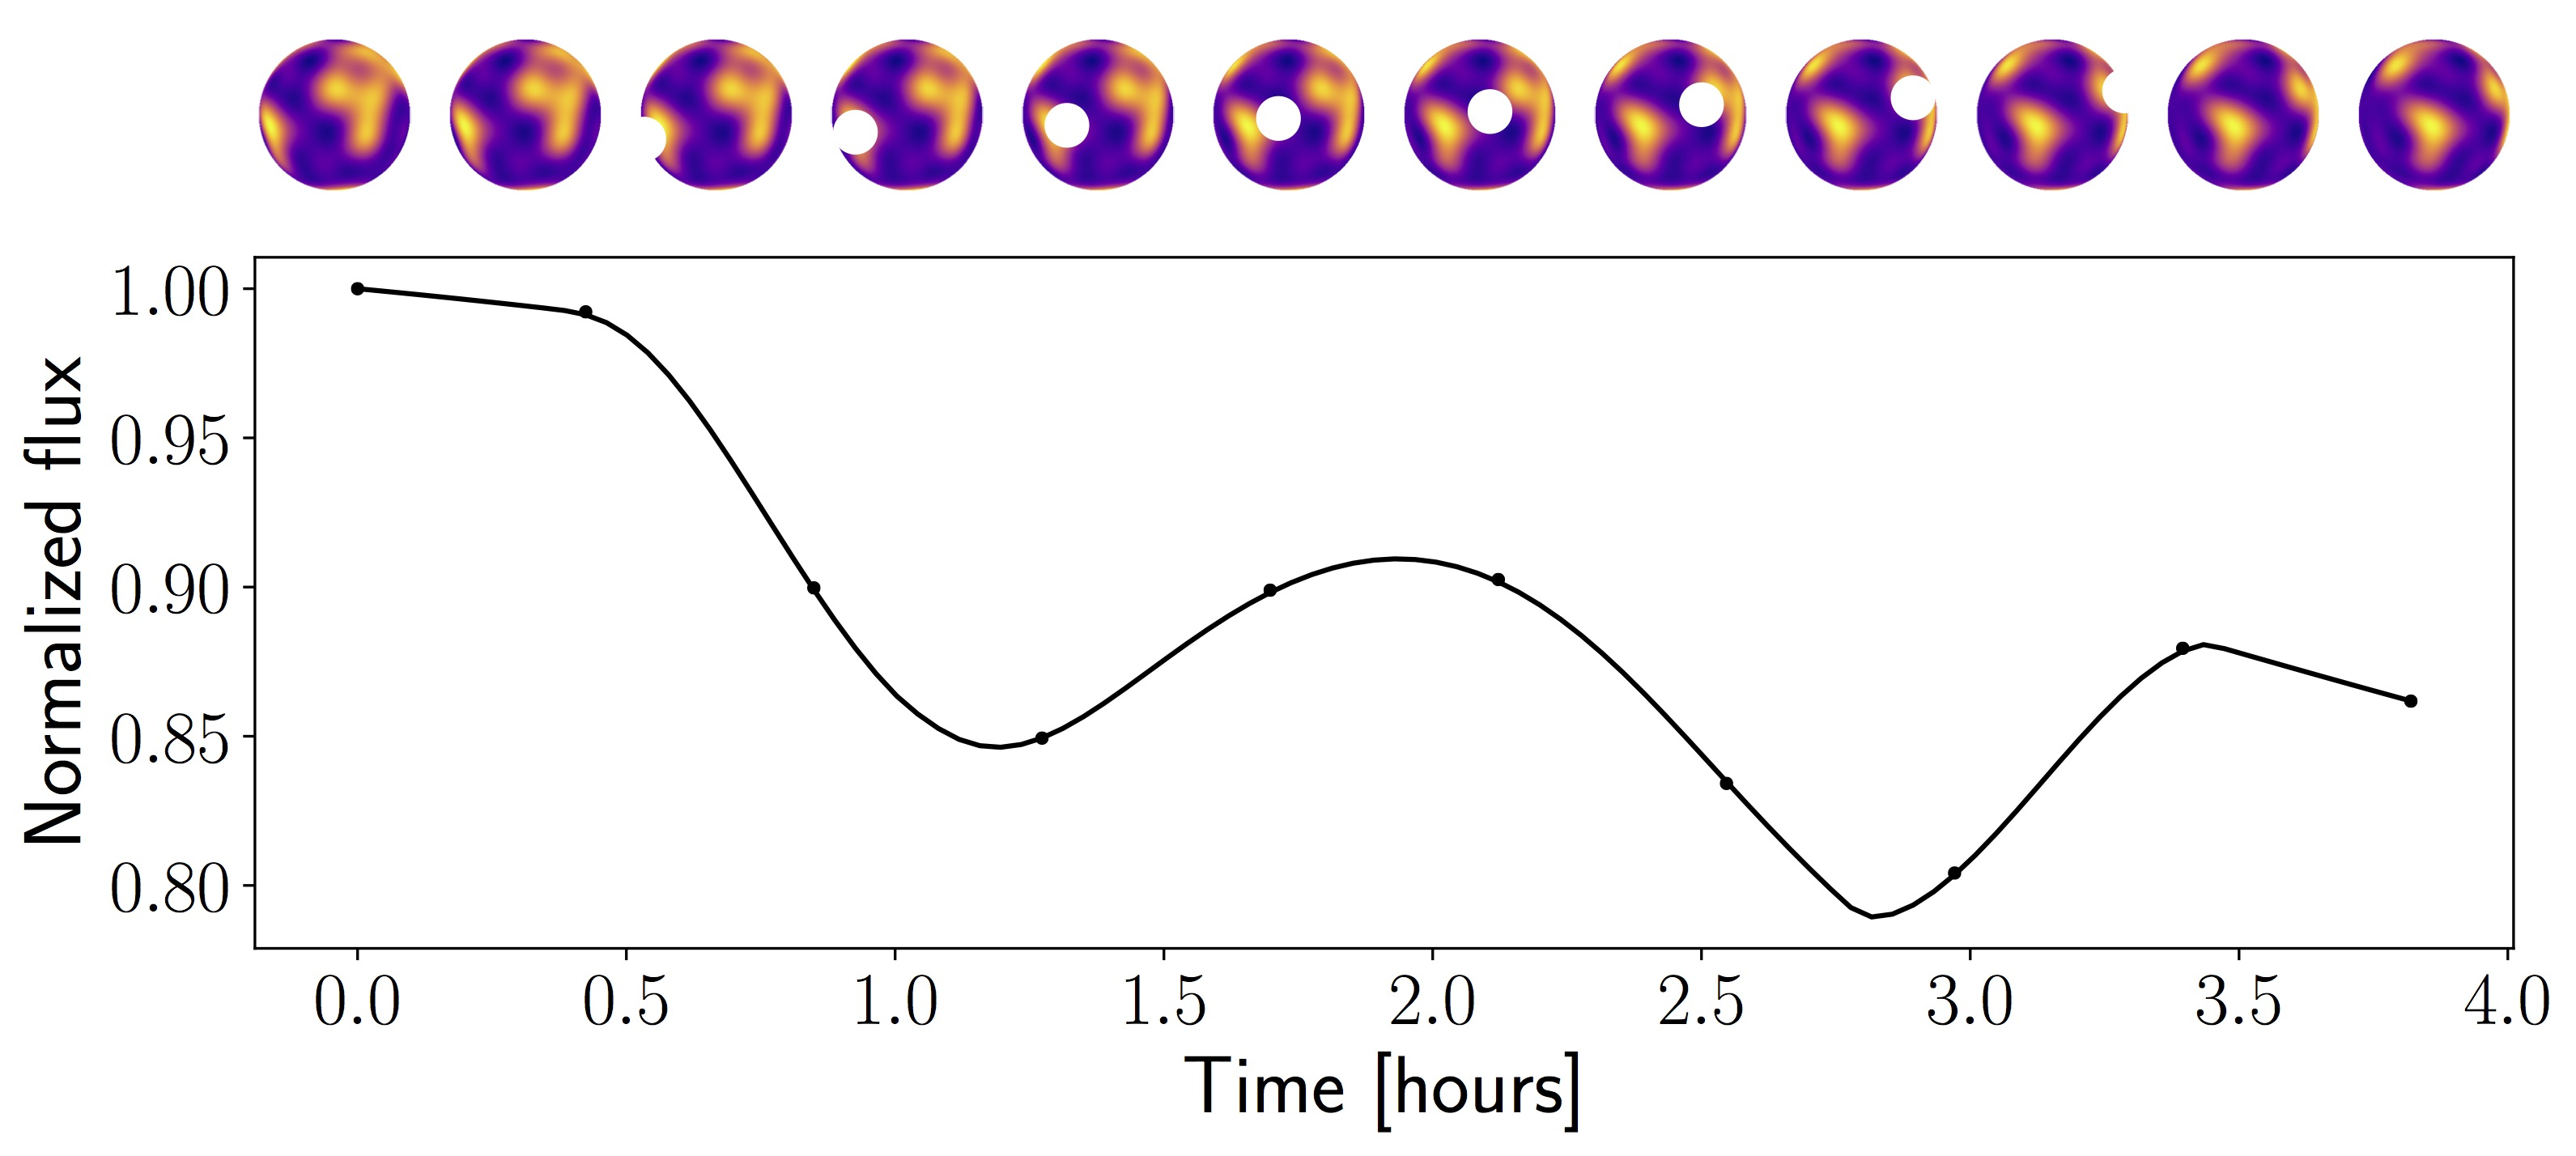
\includegraphics[width=\linewidth]{figures/earthoccultation.pdf}
    \caption{\label{fig:earthoccultation}
             \python{earthoccultation}
             Occultation light curve for the Moon transiting the
             rotating Earth,
             computed from the $l_\mathrm{max} = 10$ expansion from
             Figure~\ref{fig:earth}. The two largest dips are due
             to the occultations of South America (left) and Africa
             (right). Once again, the black dots correspond to the
             numerical solution.}
    \end{centering}
\end{figure}
%

To further illustrate the code, we return to our spherical harmonic
expansion of the Earth.
Figure~\ref{fig:earthoccultation} shows an occultation light curve
computed for a hypothetical transit of the Earth by the Moon. The
occultation lasts about four hours, during which time
the sub-observer point rotates from Africa to South America, causing a
steady flux decrease as the Pacific Ocean rotates into view. The
occultation is double-dipped: one dip due to the occultation of South
America, and one dip due to the occultation of Africa.

% ------------------------------------------------------------------------------
\subsection{Computing transits of limb-darkened stars}
\label{sec:starrytransits}
% ------------------------------------------------------------------------------

The formalism developed in this paper can easily be extended to the case
of occultations (transits) of limb-darkened stars by noting that any
radially symmetric specific intensity profile can be expressed as a sum
over the $m = 0$ spherical harmonics (see Figure~\ref{fig:ylms}).
%
In particular, \citet{limbdark} show how a limb darkening profile
that is an order $l$ polynomial function of the radial coordinate,
$\upmu = \z = \sqrt{1 - \x^2 - \y^2}$, can be exactly
expressed in terms of the $m = 0$ spherical harmonics up to order $l$.

For convenience, we implement this functionality in \starry via the
\starryLimbDarkenedMap class. This class behaves similarly
to the \starryMap class but allows users
to specify the coefficients of a limb darkening polynomial of arbirtary order
directly as follows:
%
\begin{lstlisting}[language=Python,firstnumber=last]
from starry import LimbDarkenedMap
map = LimbDarkenedMap(lmax)
map.set_coeff(1) = u1
map.set_coeff(2) = u2
...
map.set_coeff(lmax) = ulmax
\end{lstlisting}
%
or, more compactly,
\footnote{Note that \starryMap instances accept two indices
($l$ and $m$) to specify a map coefficient, while
\starryLimbDarkenedMap instances accept a single index $l$,
the limb darkening polynomial index. Note, also, that in the limb-darkened
case the $l = 0$ coefficient cannot be set, as it is automatically computed to
enforce the correct normalization.}
%
\begin{lstlisting}[language=Python,firstnumber=last]
map[1] = u1
map[2] = u2
...
map[lmax] = ulmax
\end{lstlisting}
%
where \textsf{lmax} is the order of the limb darkening polynomial.
In the case of quadratic limb darkening ($l_\mathrm{max} = 2$),
this sets the map's limb darkening profile to
%
\begin{align}
    \label{eq:quadraticld}
    \frac{I(\upmu)}{I(1)} &= 1 - u_1 (1 - \upmu) - u_2 (1 - \upmu)^2
    \quad,
\end{align}
%
with $\upmu$ given above.
From \citet{limbdark}, this corresponds to the spherical harmonic sum
%
\begin{align}
    \label{eq:qldylm}
    \frac{I(\x, \y)}{I(1)} =
            \frac{2\sqrt{\pi}}{3} (3 - 3u_1 - 4u_2) \, Y_{0,0}
          + \frac{2\sqrt{\pi}}{\sqrt{3}} (u_1 + 2u_2) \, Y_{1,0}
          - \frac{4\sqrt{\pi}}{3\sqrt{5}} u_2 \, Y_{2,0}
      \quad,
\mathematica{limbdark}
\end{align}
%
where we set
%
\begin{align}
    \label{eq:I1}
    I(1) = \frac{1}{\pi(1 - \frac{1}{3}u_1 - \frac{1}{6}u_2)}
\end{align}
%
to enforce the integral of the specific intensity over the visible disk
is unity.
At present, \starry does not support
adding limb darkening to non-radially symmetric maps; this
functionality will be added in the future to allow for limb darkening
of, say, planetary atmospheres. Note also that unlike \starryMap,
instances of \starryLimbDarkenedMap cannot be rotated.

Figure~\ref{fig:transit} shows a transit light curve computed with \starry
for $u_1 = 0.4, u_2 = 0.26$. The planet/star radius ratio is $r = 0.1$ and
the planet transits at impact parameter $b = 0.5$. For comparison, we also
compute the flux with \batman \citep{Kreidberg2015} and with a
high precision numerical integration of the surface integral of
\eq{quadraticld}. The relative error on the flux for \starry flux is less
than $10^{-7}$ parts per million everywhere in the light curve.
%
\begin{figure}[ht!]
    \begin{centering}
    \includegraphics[width=\linewidth]{figures/transit.pdf}
    \caption{\label{fig:transit}
             \python{transit}
             Sample transit light curve for a planet ($r = 0.1$) transiting a
             quadratically limb-darkened star ($u_1 = 0.4, u_2 = 0.26$). The
             top panel shows the \starry (blue curve) and \batman
             (orange dots) light curves, as well as a light curve generated
             by a high precision direct numerical integration of the surface
             integral (purple dots). The bottom panel shows the relative
             error on the flux in parts per million compared to the high
             precision numerical solution for \starry (blue) and \batman (orange).}
    \end{centering}
\end{figure}
%

% ------------------------------------------------------------------------------
\subsection{Photodynamics}
\label{sec:starryphotodynamics}
% ------------------------------------------------------------------------------

The \starryMap and \starryLimbDarkenedMap classes
discussed above are convenient when the rotational
state of the body in question and/or the position of the occultor is known,
or when these can easily be computed by some other means. For convenience,
\starry implements a simple Keplerian solver to compute stellar and
planetary light curves for exoplanet systems given the orbital parameters as
input. Users can access this functionality by instantiating a
\starryStar and any number of \starryPlanet objects, then
passing them to a \starrySystem instance. Let us begin by
creating a star:
%
\begin{lstlisting}[language=Python,firstnumber=last]
from starry import Star
star = Star(lmax=2)
\end{lstlisting}
%
A \starryStar has unit radius and unit luminosity; the planet's radii,
semi-major axes, and luminosities are all defined relative to these.
The star's \ldmap attribute is a \starryLimbDarkenedMap instance,
which by default is set to a constant term corresponding to uniform surface brightness.
We can add quadratic limb darkening as before by editing the star's \ldmap
attribute:
%
\begin{lstlisting}[language=Python,firstnumber=last,]
star.map[1] = 0.40
star.map[2] = 0.26
\end{lstlisting}
%
where we arbitrarily set $u_1 = 0.40$ and $u_2 = 0.26$.
Next, we can instantiate a planet by typing
%
\begin{lstlisting}[language=Python,firstnumber=last]
from starry import Planet
planet = Planet(lmax=1, r=0.1, L=5.e-3, porb=4.3, prot=4.3)
\end{lstlisting}
%
where \textsf{lmax} is the highest degree of the planet map, \textsf{r} is the
planet radius in units of the stellar radius, \textsf{L} is the total planet luminosity
in units of the stellar luminosity,
\textsf{porb} is the orbital period and \textsf{prot} is the rotational
period, both in days.
Several other keyword arguments may be provided; these are detailed in full
in the \href{https://rodluger.github.io/starry/starry.html\#starry.Planet}{documentation}.
As with \starryStar, the planet's map
(a \starryMap instance) can be accessed
via the \ldmap property. Suppose we wish to give the planet a simple
dipole map ($Y_{1,0}$) with peak brightness at the sub-stellar point.
\starry expects the planet map to be instantiated at an eclipsing
configuration (full phase), so we want to set the coefficient for the $Y_{1,0}$
harmonic (see Figure~\ref{fig:ylms}):
%
\begin{lstlisting}[language=Python,firstnumber=last]
planet.map[1, 0] = 0.5
\end{lstlisting}
%
Finally, care should be taken to ensure the map is positive everywhere. By default,
the coefficient of the $Y_{0,0}$ term of a planet's map is fixed at unity, since
changing this term would change the total luminosity (this should instead be
modified via the \textsf{planet.L} property). In the case of a simple dipole map of
the form $Y_{0,0} + c Y_{1, 0}$, it is easy to show that as long as we enforce
%
\begin{align}
    |c| \le \frac{1}{\sqrt{3}} \approx 0.5773
\end{align}
%
the map will be non-negative everywhere along the unit sphere.
\footnote{In Cartesian coordinates, we have $Y_{0,0} = \sqrt{\frac{1}{4\pi}}$ and
$Y_{1,0} = \sqrt{\frac{3}{4\pi}}z$. At the anti-stellar point ($z = 1$), the ratio
of these two terms is $\nicefrac{1}{\sqrt{3}}$, so the absolute value of the
coefficient of $Y_{1,0}$ must be at most this value to ensure the anti-stellar
point has a non-negative surface intensity.}
%
For more details on ensuring surface maps are positive everywhere, see
\S\ref{sec:nonnegative}.

We are now ready to instantiate the planetary system:
%
\begin{lstlisting}[language=Python,firstnumber=last]
from starry import System
system = System([star, planet])
\end{lstlisting}
%
(note that the star must always be listed first).
We can now compute the full light curve:
%
\begin{lstlisting}[language=Python,firstnumber=last]
system.compute(time)
\end{lstlisting}
%
where \textsf{time} is the array of times (in days) at which to compute the
light curve. This command internally calls the \flux method of each
of the surface maps, populating the \textsf{flux} attribute of each body
with its respective light curve. The total light curve (the sum of the
light curves of each of the bodies in the system, including the star) is
stored in \starrySystemflux. The top panel of Figure~\ref{fig:system} shows
the light curve for the system we instantiated above: both the transits
and secondary eclipses of the planet are clearly visible. For flair, we added
a hotspot offset of $15^\circ$ to simulate advection of heat by a
westward wind, causing the peak of the planet's phase curve to occur slightly
before secondary eclipse (refer to the \Python script for details).

%
\begin{figure}[ht]
    \begin{centering}
    \includegraphics[width=\linewidth]{figures/system.pdf}
    \caption{\label{fig:system}
             \python{system}
             Sample analytic exoplanet system light curves computed with \starry.
             \emph{Top:} a hot Jupiter
             transiting a Sun-like star. The planet's map is a simple dipole,
             with the hotspot offset 15$^\circ$ from stellar noon; the offset
             in the secondary eclipse from the peak of the phase curve is
             apparent. \emph{Bottom:} a two-planet system with more complex
             surface maps. In addition to transits and secondary eclipses,
             a few planet-planet occultations are visible (e.g., the very short
             events at $t=0.1$ and $t=3.4$ days).}
    \end{centering}
\end{figure}
%

The bottom panel of the figure shows a two-planet system with more elaborate
surface maps. In addition to the transits, eclipses, and complex phase curve
morphology, several planet-planet occultations are also visible in the
light curve.

% ------------------------------------------------------------------------------
\subsection{Gradients of the light curves}
\label{sec:gradients}
% ------------------------------------------------------------------------------
Since all expressions derived in this paper are analytic, so too are their
derivatives. The ability to compute derivatives of a light curve model with
respect to the model parameters can be extremely useful in both optimization
and inference problems. When fitting a model to data with an optimization
algorithm, knowledge of the gradient of the objective function can greatly
speed up convergence, as the optimizer always ``knows'' which direction to
take a step in to improve the fit. Gradients can also be used in Hamiltonian
Monte Carlo (HMC) simulations, in which the gradient of the likelihood is used
to improve the efficiency of the sampler and greatly speed up convergence of
the chains \citep[e.g.,][]{Betancourt2017}.

In principle, one could differentiate the recurrence relations in
the Appendix and arrive at expressions for the derivatives of a light curve with
respect to any of the input parameters. \citet{Pal2008} derived gradients in
this fashion for the case of transits across a quadratically limb-darkened star.
However, for the complex surface maps we consider here, differentiating all our
equations would be an extremely tedious
task. Instead, we can take advantage of the analytic nature of our expressions
and compute all derivatives using automatic differentiation \citep[autodiff; e.g.,][]{Wengert1964}.
Despite the complexity of the expressions we derive here, each of the individual
steps involved in computing a light curve is either a basic arithmetic operation
or the evaluation of an elementary function and is therefore trivially differentiable.
Autodiff algorithms exploit this fact by repeatedly applying the chain rule to
compute the derivatives of any function during its evaluation, returning derivatives
that are accurate to machine precision and at a speed that can be significantly greater
than that of numeric (or symbolic) differentiation.

We employ the autodiff algorithm of the Eigen \citep{eigen} C++ library to compute
derivatives of the flux with respect to all input parameters. Although fast,
evaluation of the derivatives introduces overhead to the computation
and is therefore disabled by default. To enable it, users should instantiate the
\starry classes from the \starrygrad module (i.e., users should use
\gradMap instead of \starryMap). The classes in this module are
identical in most respects to those in \starry, but automatically compute derivatives
whenever their methods are called. All derivatives are stored in the \textsf{gradient}
property of the class as a dictionary. As an example, let us instantiate a \gradMap
class and compute the flux at one point during an occultation:
%
\begin{lstlisting}[language=Python,firstnumber=last]
from starry.grad import Map
map = Map(1)
map[1, 0] = 1
map.flux(axis=(0, 1, 0), theta=30, xo=0.1, yo=0.1, ro=0.1)
\end{lstlisting}
%
Running the code above outputs the value of the flux, \textsf{0.8723...},
which is exactly what you'd get with \starryMap. However, behind the scenes,
\starry also computed gradients. Here's what we get when we access \textsf{map.gradient}:
%
\begin{lstlisting}[language=Python,firstnumber=last]
{'Y_{0,0}': array([0.]),
 'Y_{1,-1}': array([-0.00153499]),
 'Y_{1,0}': array([0.87233361]),
 'Y_{1,1}': array([-0.5054145]),
 'axis_x': array([0.0007675]),
 'axis_y': array([8.52090655e-20]),
 'axis_z': array([-0.00020565]),
 'ro': array([-0.27718567]),
 'theta': array([-0.00882115]),
 'xo': array([-0.0063251]),
 'yo': array([0.00134985])}
\end{lstlisting}
%
These are the gradients of the flux with respect to each of the four map
coefficients, the three components of the rotation axis, the occultor radius,
the rotational phase, and the $xy$ position of the occultor.
%
\begin{figure}[p!]
    \begin{centering}
    \includegraphics[width=0.9\linewidth]{figures/autodiff.pdf}
    \caption{\label{fig:autodiff}
             \python{autodiff}
             Transit (top left) and secondary eclipse (top right) of a mildly
             eccentric, slightly inclined, quickly-rotating hot Jupiter with a
             dipole map, computed with \gradMap. All calls to the \gradflux
             and \gradeval methods of the maps in \starrygrad automatically
             compute derivatives with respect to all input parameters. Derivatives
             as a function of time for several of these parameters are plotted in
             orange below each light curve. From top to bottom, the curves correspond
             to derivatives with respect to time, planet radius, planet luminosity,
             orbital period, eccentricity, inclination, longitude of pericenter,
             rotational period, five of the planet surface map coefficients, and
             the linear and quadratic stellar limb darkening coefficients.
             }
    \end{centering}
\end{figure}
%
Figure~\ref{fig:autodiff} shows an example of the autodiff capabilities of
\starry for a transit and a secondary eclipse of a hot Jupiter.

% ------------------------------------------------------------------------------
\subsection{Benchmarks}
\label{sec:starrybenchmarks}
% ------------------------------------------------------------------------------

We validate all our calculations of rotational phase curves and occultation
light curves by comparing them to numerical solutions of the corresponding
surface integrals. We integrate the specific intensity of the body by
discretely summing over its surface map on an adaptive radial mesh whose
resolution is iteratively increased wherever the spatial gradient of the
%
\animation{adaptive}
%
specific intensity is large and in the vicinity of the limb of the occultor.
Click on the link at right for an animation of our adaptive mesh scheme.

%In \starry, users can request numerical solutions to the flux by typing
%
%\begin{lstlisting}[language=Python,firstnumber=last]
%F = map._flux_numerical(..., tol=1.e-4)
%\end{lstlisting}
%
%where \textsf{tol} is the error tolerance, the maximum absolute value of the
%difference between the
%specific intensity at the center of a grid cell to the average of the specific
%intensity at the four vertices of the same cell. The mesh is locally
%refined until the requested tolerance is met in all cells.

All light curves in Figure~\ref{fig:ylmlightcurves} show the flux computed
in this way as the small points along each of the curves. We find that our
analytic light curves agree with the numerical solutions to within the error
of the latter.

% ------------------------------------------------------------------------------
\subsection{Speed tests}
\label{sec:starryspeed}
% ------------------------------------------------------------------------------

Figure~\ref{fig:compare_to_numerical} shows the evaluation time for
occultation calculations as a function of the spherical
harmonic degree $l$ of the map. Analytic solutions computed with \starry
are shown as the blue dots (purple dots for \starrygrad). Also shown are calculations using the adaptive
mesh technique described in the previous section (orange dots),
brute-force integration on a 300$\times$300 Cartesian grid (green dots),
and numerical evaluation of the double integral using the
\textsf{scipy.integrate.dblquad} \citep{scipy} routine (red). The size of each point
is proportional to the log of the fractional error relative to the
\starry solution. Light curve computation using \starry is several orders of
magnitude faster and more accurate than any other evaluation technique.

Figure~\ref{fig:speed} shows the evaluation time for \starry
as a function of the number of points in the light curve for phase curves
(left) and occultation light curves (right). The top panel shows curves for
maps of different degree $l$, and the bottom panel shows curves for single-order
maps of degree $l = 5$. Evaluation time scales exponentially with increasing
degree, but \starry can compute full occultation light curves for $l = 5$ maps
with $10^5$ points in under one second. Evaluation time is roughly constant
across the different orders at fixed degree.
In Figure~\ref{fig:speed_batman} we show a speed comparison
to the \batman transit package \citep{Kreidberg2015} for transits across a
quadratically limb-darkened star. \starry is as efficient as \batman at
computing transit light curves.

\begin{figure}[ht!]
    \begin{centering}
    \includegraphics[width=0.9\linewidth]{figures/compare_to_numerical.pdf}
    \caption{\label{fig:compare_to_numerical}
             \python{speed}
             Evaluation time for a single occultation calculation as a function
             of the spherical harmonic degree of the map using
             \starry (blue), \starrygrad (purple), the adaptive mesh technique (\S\ref{sec:starrybenchmarks}, orange),
             brute force integration on a Cartesian grid (green), and
             \textsf{scipy}'s \textsf{dblquad} two-dimensional numerical
             integration routine (red).
             The size of each point is proportional to the log of the error relative
             to the \starry analytic solution.
             }
    \end{centering}
\end{figure}

\begin{figure}[p!]
    \begin{centering}
    \includegraphics[width=\linewidth]{figures/speed.pdf}
    \caption{\label{fig:speed}
             \python{speed}
             Speed tests for \starry, showing the light curve evaluation time
             as a function of number of light curve points for rotational
             phase curves (left) and occultation light curves (right) of individual
             spherical harmonics. The top
             panels show the evaluation time for spherical harmonics of different
             degrees $l$, averaged over all orders $m$. The bottom panels
             show the evaluation time for each of the positive orders
             of the $l = 5$ spherical harmonics.
             }
    \end{centering}
\end{figure}

\begin{figure}[p!]
    \begin{centering}
    \includegraphics[width=0.65\linewidth]{figures/speed_batman.pdf}
    \caption{\label{fig:speed_batman}
             \python{speed_batman}
             Speed comparison to the \batman transit modeling package
             \citep{Kreidberg2015} for a hot Jupiter transit across a
             quadratically limb-darkened star.
             }
    \end{centering}
\end{figure}

% ==============================================================================
% ------------------------------------------------------------------------------
% ------------------------------------------------------------------------------
\section{Caveats}
\label{sec:caveats}
% ------------------------------------------------------------------------------
% ------------------------------------------------------------------------------
% ==============================================================================

\subsection{Wavelength dependence}
In our formalism thus far we have avoided mention of wavelength dependence
of a body's surface map. In our derivations we treated the specific intensity at a point
on the body's map as a scalar: a single number corresponding to the total power
emitted to space by an infinitesimal area element on the body's surface.
When applying \starry to actual data, this intensity can either
be the power integrated over a range of wavelengths, in which case the light curve
has units of flux proper,
corresponding to (say) the quantity measured by an instrument performing filter
photometry; or the power at a \emph{specific} wavelength, in which case the light curve
computed by \starry has units of \emph{spectral} flux, corresponding to (say) the
flux measured in a tiny wavelength bin by a spectrometer. Note, importantly,
that in the former case the ``surface map'' is in reality the integral of the body's
wavelength-dependent specific intensity convolved with the instrument's spectral
response function over a given wavelength range. While \starry can be used to
compute wavelength-dependent light curves by specifying a different map
for each wavelength, this is at present inefficient, since \starry re-computes
the occultation integrals for each wavelength bin. The next version of \starry
will include functionality to allow users to easily and quickly compute
spectra of celestial bodies in occultation.

\subsection{Reflectance light curves}
At present, \starry can only compute thermal phase curves and occultation
light curves for planets and moons. Reflectance light curves are significantly
more difficult to compute analytically because of the sharp discontinuity in the
illumination gradient at the terminator. In principle, the stellar illumination
pattern could be modeled with a high order spherical harmonic expansion, but
this approach cannot accurately capture the sharp day/night transition at the
terminator and typically leads to spurious ringing on the night side. A
better approach is to treat the terminator as one of the boundaries of the
surface integral and use Green's theorem to compute the line integral about
this elliptical curve. This will be the topic of a future paper and will
be implemented in future versions of the code.

\subsection{Non-negative surface maps}
\label{sec:nonnegative}
While spherical harmonics are a convenient way to approximate surface
maps of celestial bodies, it is not trivial to ensure
that a given spherical harmonic expansion $\bvec{y}$ evaluates to
non-negative values everywhere on the unit sphere. This is because
there is no analytic way to compute the extrema of a function of
spherical harmonics of arbitrary order.
This fact makes it difficult to enforce the physical prior that the
specific intensity of a celestial body cannot be negative, which
could be desirable when fitting a model to real data. The minimum
can, of course, be found numerically, although this is slow and
should probably not be done repeatedly during optimization to
enforce a prior. Nevertheless, users can find the minimum of the
map over the entire domain by typing
%
\begin{lstlisting}[language=Python,firstnumber=last]
map.minimum()
\end{lstlisting}
%
This method evaluates the surface map on a coarse grid, locates the
approximate location of the minimum, and performs a gradient-descent
optimization to locate the global minimum of the map. If the minimum
is negative, users should either scale the $Y_{0,0}$ coefficient up
or the coefficients of all other harmonics down until the map is
non-negative everywhere.

\subsection{Very large occultors}
When the occultor becomes much larger than the occulted body ($r_o \gg 1$),
the analytic solutions to the occultation integrals may become numerically
unstable when the map degree $l$ is large. This is due to the propagation of
round-off error in the recurrence relations, which we mitigate
with careful Taylor expansions and reparameterizations of the equations.
We discuss this at length in Appendix~\ref{app:numericalstability}.
In general, numerical stability is
not likely to be an issue for $l \leq 8$ and $r_o \lesssim 500$, for which
the maximum fractional error due to round-off is on the order of one part
per thousand, which in the case of exoplanets is likely far below the
detectability limits of telescopes in the foreseable future. Nevertheless, users
can bypass these numerical issues by instantiating a map from the \textsf{starry.multi}
module:
%
\begin{lstlisting}[language=Python,firstnumber=last]
map = starry.multi.Map()
\end{lstlisting}
%
to enable multiprecision mode, which by default is set to quadruple (128-bit)
floating point precision. We caution, however, that this will increase
computation time by at least an order of magnitude.

\subsection{Three-body events}
The occultation formalism developed in this paper applies specifically to the
case of a single occultor, so \starry cannot at present handle mutual occultations
involving more than two bodies. However, even for an arbitrary number of bodies
the problem is still analytic, since Green's theorem may be employed in the same
way, but instead evaluating the line integrals along the more complex network of
arcs defining the edges of the visible portion of the body's surface. This was
first noted by \cite{Pal2012}, whose \textsf{mttr} code computes analytic
transit light curves for mutually overlapping bodies such as a transiting
planet with a moon. Future versions of \starry will extend the calculations
to this general case.

% ==============================================================================
% ------------------------------------------------------------------------------
% ------------------------------------------------------------------------------
\section{Conclusions}
\label{sec:conclusions}
% ------------------------------------------------------------------------------
% ------------------------------------------------------------------------------
% ==============================================================================

In this paper, we derived a formalism to compute analytic thermal light curves of celestial
bodies in occultation, provided their specific intensity maps can be expressed as a sum
of spherical harmonics. Our expressions extend the analytic results of the
\citet{MandelAgol2002} transit model for limb-darkened stars to transits and
occultations of celestial bodies whose surface maps are not radially symmetric
and/or possess higher order features, and are thus generally applicable to
stars, planets, and moons. We derived recurrence relations to quickly compute
occultation light curves for surface maps expressed at arbitrary spherical harmonic degree.
We showed, in particular, that the flux contribution from higher degree terms
depends on the same elliptic integrals as the linear limb darkening term,
so these need only be evaluated once per light curve cadence. This results in
evaluation times for higher degree maps that are extremely fast, and
only marginally slower than in the quadratic limb-darkening case.
In the limit of zero occultor size, our expressions trivially reduce to equations
for thermal phase curves of celestial bodies.

We introduced \starry, a \Python-wrapped model coded in \cpp
that can be used to compute phase curves and occultation light curves for
individual celestial bodies or entire exoplanet systems. \starry computes
transits, secondary eclipses, phase curves, and planet-planet occultations
analytically and is comparable in speed to other transit-modeling packages such
as \batman \citep{Kreidberg2015}. Because the light curves are all analytic,
\starry can also easily compute analytic gradients of the light curves with respect
to all input parameters via autodifferentiation, facilitating its interface with
gradient-based inference schemes such as Hamiltonian Monte Carlo (HMC)
or gradient-descent optimization methods.

Although we have in mind the application of this \starry to exoplanets, it could
in principle be applied to eclipsing binaries as well.  If the deformation of
the body is small and reflection is negligible, as is the case for long orbital periods,
then the surface brightness of each star can be decomposed into spherical harmonics,
and the \starry formalism may be used to integrate their phase curves and eclipses.
One could imagine applying \starry, for instance, to secondary eclipses of white
dwarfs to search for non-uniform surface brightness.

At present, \starry supports only
monochromatic surface maps, making it ideally suited for the modeling of
light curves collected via filter photometry, but future work will extend
it to spectrophotometry. \starry is also limited to thermal light curves of
planets and moons, since the discontinuity in the gradient of the
illumination pattern at the terminator makes it more challenging to analytically
solve the surface integrals in reflected light. However, an analytic solution
is likely to exist, and future work aims to extend \starry to this case.

The upcoming James Webb Space Telescope (JWST) and eventual
next-generation telescopes such as the Origins Space Telescope (OST) will
measure exoplanet secondary eclipses and
phase curves in the thermal infrared to unprecedented precision. \starry
can compute extremely fast and high-precision models for these
light curves, enabling the reconstruction of two-dimensional maps of these
alien worlds.


\acknowledgments
This work was supported by the NASA Astrobiology
Institute's Virtual Planetary Laboratory under Cooperative
Agreement number NNA13AA93A.
%
Some of the results in this paper have been derived using the HEALPix
\citep{Gorski2005} package.



%
\bibliography{starry}
%


% ==============================================================================
% ------------------------------------------------------------------------------
% ------------------------------------------------------------------------------
\pagebreak
\appendix
% ------------------------------------------------------------------------------
% ------------------------------------------------------------------------------
% ==============================================================================


% ==============================================================================
% ------------------------------------------------------------------------------
% ------------------------------------------------------------------------------
\section{Spherical harmonics}
\label{app:spharm}
% ------------------------------------------------------------------------------
% ------------------------------------------------------------------------------
% ==============================================================================

In spherical coordinates, the spherical harmonics may be compactly represented
as in Equation~(\ref{eq:ylmtp}). The formalism in this paper requires us to express
them in Cartesian form, which is somewhat more cumbersome but still tractable.
%
Using Equation~(\ref{eq:xyz}) and expanding Equation~(\ref{eq:ylmtp})
via the multiple angle formula, we obtain
%
\begin{align}
    \label{eq:ylm0}
    Y_{lm}(\x, \y , \z) =
    \left(\frac{1}{\sqrt{1 - \z^2}}\right)^{|m|}
    \begin{dcases}
        \bar{P}_{lm}(\z)
        \sum_{j\, \mathrm{even}}^{m}
        \left(-1\right)^\frac{j}{2}
        \binom{m}{j}
        \x^{m - j}
        \y^j
         & \qquad m \geq 0
         %
         \\[1em]
         %
        \bar{P}_{l|m|}(\z)
        \sum_{j\, \mathrm{odd}}^{|m|}
        \left(-1\right)^\frac{j-1}{2}
        \binom{|m|}{j}
        \x^{|m| - j}
        \y^j
        & \qquad m < 0 \quad ,
    \end{dcases}
\end{align}
%
where $\binom{\bigdot}{\bigdot}$ is the binomial
coefficient. The normalized associated Legendre functions are defined as
%
\begin{align}
    \label{eq:plm}
    \bar{P}_{lm}(\z) &= A_{lm} \left(\sqrt{1-\z^2}\right)^m
                       \frac{\dd^m}{\dd \z^m}
                       \left[
                       \frac{1}{2^l l!}
                       \frac{\dd^l}{\dd \z^l}
                       \left(
                       \z^2 - 1
                       \right)^l
                       \right] \quad,
\end{align}
%
where
%
\begin{align}
    \label{eq:alm}
    A_{lm} = \sqrt{\frac{(2 - \delta_{m0})(2l + 1)(l - m)!}{4\pi(l + m)!}}
             \quad.
\end{align}
%
Expanding out the $\z$ derivatives, we obtain
%
\begin{align}
    \label{eq:plm_exp}
    \bar{P}_{lm}(\z) &= A_{lm} \left(\sqrt{1-\z^2}\right)^m\sum_{k=0}^{l-m}
                       \frac{2^l \left(\frac{l + m + k - 1}{2}\right)!}
                            {k!(l-m-k)!
                             \left(\frac{-l + m + k - 1}{2}\right)!}
                       \z^k
                       \quad,
\end{align}
%
which we combine with the previous results to write
%
\begin{align}
    \label{eq:ylmxyz}
    Y_{lm}(\x, \y , \z) &=
    \begin{dcases}
        \sum_{j\, \mathrm{even}}^m\sum_{k=0}^{l-m}
        \left(-1\right)^{\frac{j}{2}}
        A_{lm}
        B_{lm}^{jk}
        \x^{m - j}
        \y^j
        \z^k
        \qquad & m \ge 0 \\
        %
        \sum_{j\, \mathrm{odd}}^{|m|}\sum_{k=0}^{l-|m|}
        \left(-1\right)^{\frac{j-1}{2}}
        A_{l|m|}
        B_{l|m|}^{jk}
        \x^{|m| - j}
        \y^j
        \z^k
        \qquad & m < 0
    \end{dcases}
    \mathematica{Y}
\end{align}
%
where
%
\begin{align}
    \label{eq:blmjk}
    B_{lm}^{jk} =
    \frac{2^l m! \left(\frac{l + m + k - 1}{2}\right)!}
         {j! k! (m - j)! (l - m - k)!
          \left(\frac{-l + m + k - 1}{2}\right)!} \quad.
\end{align}
%
Since we are confined to the surface of the unit sphere, we have
$\z = \sqrt{1 - \x^2 - \y^2}$ and we may expand $\z^k$ using
the binomial theorem:
%
\begin{align}
    \z^{k} &= (1 - \x^2 - \y^2)^\frac{k}{2} \nonumber \\[0.5em]
          &=
          \begin{dcases}
              \sum_{p\,\mathrm{even}}^{k}
              \sum_{q\,\mathrm{even}}^p
              (-1)^\frac{p}{2}
              C_{pq}^{k}
              \x^{p-q} \y^{q}
              \qquad & k\,\mathrm{even} \\
              %
              \sum_{p\,\mathrm{even}}^{k - 1}
              \sum_{q\,\mathrm{even}}^p
              (-1)^\frac{p}{2}
              C_{pq}^{k-1}
              \x^{p-q} \y^{q} \sqrt{1 - \x^2 - \y^2}
              \qquad & k\,\mathrm{odd} \quad,
          \end{dcases}
          \label{eq:zk}
\end{align}
%
where
%
\begin{align}
    \label{eq:ckpq}
    C_{pq}^{k} =
    \frac{\left(\frac{k}{2}\right)!}{\left(\frac{q}{2}\right)!
    \left(\frac{k-p}{2}\right)! \left(\frac{p-q}{2}\right)!} \quad.
\end{align}
%
This gives us an expression for the spherical harmonics $Y_{lm}$
as a function of $\x$ and $\y$ only:
%
\begin{align}
    \label{eq:ylmxy}
    \mathematica{Y}
    Y_{lm}(\x, \y) &=
    \begin{dcases}
        \!\begin{aligned}%[b]
            &
                \sum_{j\, \mathrm{even}}^m
                \sum_{k\, \mathrm{even}}^{l-m}
                \sum_{p\,\mathrm{even}}^{k}
                \sum_{q\,\mathrm{even}}^p
                \left(-1\right)^{\frac{j+p}{2}}
                A_{lm}
                B_{lm}^{jk}
                C_{pq}^{k}
                \x^{m - j + p - q}
                \y^{j + q}
            \, + \\
            &
                \sum_{j\, \mathrm{even}}^m
                \sum_{k\, \mathrm{odd}}^{l-m}
                \sum_{p\,\mathrm{even}}^{k - 1}
                \sum_{q\,\mathrm{even}}^p
                \left(-1\right)^{\frac{j+p}{2}}
                A_{lm}
                B_{lm}^{jk}
                C_{pq}^{k - 1}
                \x^{m - j + p - q}
                \y^{j + q}
                \z
       \end{aligned}
       &
       \quad m \ge 0 \\
       %
       %
       \\
       %
       %
       \!\begin{aligned}%[b]
           &
               \sum_{j\, \mathrm{odd}}^{|m|}
               \sum_{k\, \mathrm{even}}^{l-|m|}
               \sum_{p\,\mathrm{even}}^{k}
               \sum_{q\,\mathrm{even}}^p
               \left(-1\right)^{\frac{j+p-1}{2}}
               A_{l|m|}
               B_{l|m|}^{jk}
               C_{pq}^{k}
               \x^{|m| - j + p - q}
               \y^{j + q}
           \, + \\
           &
               \sum_{j\, \mathrm{odd}}^{|m|}
               \sum_{k\, \mathrm{odd}}^{l-|m|}
               \sum_{p\,\mathrm{even}}^{k - 1}
               \sum_{q\,\mathrm{even}}^p
               \left(-1\right)^{\frac{j+p-1}{2}}
               A_{l|m|}
               B_{l|m|}^{jk}
               C_{pq}^{k - 1}
               \x^{|m| - j + p - q}
               \y^{j + q}
               \z
      \end{aligned}
      &
      \quad m < 0
   \end{dcases}
    %
\end{align}
%
where $\z = \z(\x, \y) = \sqrt{1 - \x^2 - \y^2}$. Evaluating the nested sums
may be computationally slow, but these operations need only be performed a
single time to construct our change of basis matrix (following section).

% ==============================================================================
% ------------------------------------------------------------------------------
% ------------------------------------------------------------------------------
\section{Change of Basis}
\label{app:basis}
% ------------------------------------------------------------------------------
% ------------------------------------------------------------------------------
% ==============================================================================

In this section we discuss how to compute the change of basis matrices
$\AOne$ and $\ATwo$ from \S\ref{sec:basis} and provide links to
\Mathematica scripts to compute them.
%
Recall that the columns of the change of basis matrix from spherical
harmonics to polynomials, $\AOne$, are just the polynomial vectors
corresponding to each of the spherical harmonics in \eq{by}. From
Equations (\ref{eq:bp}) and (\ref{eq:ylmxy}), we can calculate
the first few spherical harmonics and their corresponding polynomial vectors:
%
\begin{equation}
\def\arraystretch{1.3}
\begin{array}{@{}lcccccccl@{}}
    \phantom{..}
    Y_{0,0} = \frac{1}{2\sqrt{\pi}}
    & & & & & & & &
    \bvec{p} = \frac{1}{2\sqrt{\pi}}
                  \begin{pmatrix}
                        1 & 0 & 0 & 0 & \cdot\cdot\cdot
                  \end{pmatrix}^\mathsf{T}
    %
    \\
    %
    Y_{1,-1} = \frac{\sqrt{3}}{2\sqrt{\pi}}\y
    & & & & & & & &
    \bvec{p} = \frac{1}{2\sqrt{\pi}}
                  \begin{pmatrix}
                        0 & 0 & 0 & \sqrt{3} & \cdot\cdot\cdot
                  \end{pmatrix}^\mathsf{T}
    %
    \\
    %
    \phantom{..}
    Y_{1,0} = \frac{\sqrt{3}}{2\sqrt{\pi}}\z
    & & & & & & & &
    \bvec{p} = \frac{1}{2\sqrt{\pi}}
                \begin{pmatrix}
                      0 & 0 & \sqrt{3} & 0 & \cdot\cdot\cdot
                \end{pmatrix}^\mathsf{T}
    %
    \\
    %
    \phantom{..}
    Y_{1,1} = \frac{\sqrt{3}}{2\sqrt{\pi}}\x
    & & & & & & & &
    \bvec{p} = \frac{1}{2\sqrt{\pi}}
                  \begin{pmatrix}
                        0 & \sqrt{3} & 0 & 0 & \cdot\cdot\cdot
                  \end{pmatrix}^\mathsf{T}
    %
    \\
    %
    Y_{2,-2} = \cdot\cdot\cdot
    & & & & & & & &
    \bvec{p} = \cdot\cdot\cdot
\end{array}
\end{equation}
%
From these we can construct $\AOne$. As an example, for spherical
harmonics up to degree $l_\mathrm{max} = 2$, this is
%
\begin{equation}
    \label{eq:AOne}
    \setstackgap{L}{1.25\baselineskip}
    \fixTABwidth{T}
    \AOne =
    \frac{1}{2 \sqrt{\pi }}
        \parenMatrixstack{
            1 & 0 & 0 & 0 & 0 & 0 & \sqrt{5} & 0 & 0 \\
            0 & 0 & 0 & \sqrt{3} & 0 & 0 & 0 & 0 & 0 \\
            0 & 0 & \sqrt{3} & 0 & 0 & 0 & 0 & 0 & 0 \\
            0 & \sqrt{3} & 0 & 0 & 0 & 0 & 0 & 0 & 0 \\
            0 & 0 & 0 & 0 & 0 & 0 & -\frac{3 \sqrt{5}}{2} & 0 & \frac{\sqrt{15}}{2} \\
            0 & 0 & 0 & 0 & 0 & 0 & 0 & \sqrt{15} & 0 \\
            0 & 0 & 0 & 0 & \sqrt{15} & 0 & 0 & 0 & 0 \\
            0 & 0 & 0 & 0 & 0 & \sqrt{15} & 0 & 0 & 0 \\
            0 & 0 & 0 & 0 & 0 & 0 & -\frac{3 \sqrt{5}}{2} & 0 & -\frac{\sqrt{15}}{2}
        }\quad.
    \mathematica{A1}
\end{equation}
%

We compute the change of basis matrix from polynomials to Green's
polynomials, $\ATwo$, in a similar manner. In practice,
it is easier to express the elements of the Green's basis $\gbasis$ in terms
of the elements of the polynomial basis $\pbasis$ and use those to populate the
columns of the matrix $\ATwo^{-1}$. Continuing our example
for $l_\mathrm{max} = 2$, our second change of basis matrix
is
%
\begin{equation}
    \setstackgap{L}{1.1\baselineskip}
    \fixTABwidth{T}
    \ATwo =
        \parenMatrixstack{
            \quad\quad\, 1\, \quad\quad\quad\quad & 0 & 0 & 0 & 0 & 0 & 0 & 0 & 0 \\
            0 & \frac{1}{2} & 0 & 0 & 0 & 0 & 0 & 0 & 0 \\
            0 & 0 & 1 & 0 & 0 & 0 & 0 & 0 & 0 \\
            0 & 0 & 0 & 1 & 0 & 0 & 0 & 0 & 0 \\
            0 & 0 & 0 & 0 & \frac{1}{3} & 0 & 0 & 0 & 0 \\
            0 & 0 & 0 & 0 & 0 & -\frac{1}{3} & 0 & 0 & 0 \\
            0 & 0 & 0 & 0 & 0 & 0 & \frac{1}{2} & 0 & 0 \\
            0 & 0 & 0 & 0 & 0 & 0 & 0 & \frac{1}{3} & 0 \\
            0 & 0 & 0 & 0 & 0 & 0 & 0 & 0 & 1
        }\quad.
    \mathematica{A2}
\end{equation}
%

Finally, recall that the complete change of basis matrix from spherical
harmonics to Green's polynomials, $\bvec{A}$, is just the matrix product
of $\ATwo$ and $\AOne$. For $l_\mathrm{max} = 2$, we have
%
\begin{equation}
    \mathematica{A}
    \setstackgap{L}{1.25\baselineskip}
    \fixTABwidth{T}
    \bvec{A} =
        \frac{1}{2\sqrt{\pi}}
        \parenMatrixstack{
        1 & 0 & 0 & 0 & 0 & 0 & \sqrt{5} & 0 & 0 \\
        0 & 0 & 0 & \frac{\sqrt{3}}{2} & 0 & 0 & 0 & 0 & 0 \\
        0 & 0 & \sqrt{3} & 0 & 0 & 0 & 0 & 0 & 0 \\
        0 & \sqrt{3} & 0 & 0 & 0 & 0 & 0 & 0 & 0 \\
        0 & 0 & 0 & 0 & 0 & 0 & -\frac{\sqrt{5}}{2} & 0 & \frac{\sqrt{\frac{5}{3}}}{2} \\
        0 & 0 & 0 & 0 & 0 & 0 & 0 & -\sqrt{\frac{5}{3}} & 0 \\
        0 & 0 & 0 & 0 & \frac{\sqrt{15}}{2} & 0 & 0 & 0 & 0 \\
        0 & 0 & 0 & 0 & 0 & \sqrt{\frac{5}{3}} & 0 & 0 & 0 \\
        0 & 0 & 0 & 0 & 0 & 0 & -\frac{3 \sqrt{5}}{2} & 0 & -\frac{\sqrt{15}}{2}
        }\quad.
\end{equation}
%

% ==============================================================================
% ------------------------------------------------------------------------------
% ------------------------------------------------------------------------------
\vspace*{4em}
\section{Rotation of spherical harmonics}
\label{app:rotation}
% ------------------------------------------------------------------------------
% ------------------------------------------------------------------------------
% ==============================================================================

% ------------------------------------------------------------------------------
\subsection{Euler angles}
\label{app:euler}
% ------------------------------------------------------------------------------

\citet{AlvarezCollado1989} derived expressions for the rotation matrices for
the real spherical harmonics of a given degree $l$ from the corresponding
complex rotation matrices \citep{Steinborn1973}:
%
\begin{align}
    \label{eq:rl}
    \bvec{R}^l = \bvec{U}^{-1} \bvec{D}^l \bvec{U}
\end{align}
%
where
%
\begin{align}
    \label{eq:dl}
    \bvec{D}^l_{m,m'} &= \mathrm{e}^{-\ii (\alpha m' + \gamma m)}
                       (-1)^{m' + m}
                       \sqrt{
                            (l - m)! (l + m)! (l - m')! (l + m')!
                       }
                       \nonumber \\
                       & \phantom{=}
                       \times
                       \sum_k (-1)^k
                              \frac{
                                \cos\left(\frac{\beta}{2}\right)^{2l + m - m' - 2k}
                                \sin\left(\frac{\beta}{2}\right)^{-m + m' + 2k}
                              }{
                                k! (l + m - k)! (l - m' - k)! (m' - m + k)!
                              }
\end{align}
%
is the rotation matrix for the complex spherical harmonics of degree $l$ and
%
\begin{equation}
    \label{eq:U}
    \setstackgap{L}{1.25\baselineskip}
    \fixTABwidth{T}
    \bvec{U} =
    \frac{1}{\sqrt{2}}
        \parenMatrixstack{
            \quad\quad\, \ddots \, \quad\quad\quad\quad
                   &     &     &     &          &     &     &     & \Ddots \\
                   & \ii &     &     &          &     &     &  1  &        \\
                   &     & \ii &     &          &     &  1  &     &        \\
                   &     &     & \ii &          &  1  &     &     &        \\
                   &     &     &     & \sqrt{2} &     &     &     &        \\
                   &     &     & \ii &          & -1  &     &     &        \\
                   &     & -\ii&     &          &     &  1  &     &        \\
                   & \ii &     &     &          &     &     & -1  &        \\
            \Ddots &     &     &     &          &     &     &     & \ddots
        }\quad.
\end{equation}
%
describes the transformation from complex to real spherical harmonics. In
\eq{dl} above, $\alpha$, $\beta$, and $\gamma$ are the (proper) Euler angles
for rotation in the $z-y-z$ convention.
%
To obtain a rotation matrix for an arbitrary vector $\bvec{y}$ with spherical
harmonics of different orders up to $l = l_\mathrm{max}$, we define the
block-diagonal matrix $\bvec{R}$:
%
\begin{equation}
    \label{eq:rblockdiag}
    \setstackgap{L}{1.25\baselineskip}
    \fixTABwidth{T}
    \bvec{R} =
        \parenMatrixstack{
            \quad\quad \, \bvec{R}^0 \, \quad\quad
                       &            &            &            &  \\
                       & \bvec{R}^1 &            &            &  \\
                       &            & \bvec{R}^2 &            &  \\
                       &            &            & \bvec{R}^3 &  \\
                       &            &            &            & \ddots
        }\quad.
    \mathematica{R}
\end{equation}
%
Rotation of $\bvec{y}$ by the Euler angles $\alpha$, $\beta$, and $\gamma$
is performed via \eq{rotation} with $\bvec{R}$ given by \eq{rblockdiag}.

% ------------------------------------------------------------------------------
\subsection{Axis-angle}
\label{app:axisangle}
% ------------------------------------------------------------------------------

It is often more convenient to define a rotation by an axis $\bvec{u}$
and an angle $\theta$ of rotation about that axis. Given a unit vector
$\bvec{u}$ and an angle $\theta$, we can find the corresponding Euler
angles by comparing the 3-dimensional Cartesian rotation matrices for
both systems,
%
\begin{equation}
    \label{eq:rotP}
    \setstackgap{L}{1.25\baselineskip}
    \fixTABwidth{T}
    \mathbf{P} =
        \parenMatrixstack{
        c_\theta + u_x^2 \left(1 - c_\theta\right)
        &
        u_x u_y \left(1 - c_\theta\right) - u_z s_\theta
        &
        u_x u_z \left(1 - c_\theta\right) + u_y s_\theta
        \\
        u_y u_x \left(1 - c_\theta\right) + u_z s_\theta
        &
        c_\theta + u_y^2\left(1 - c_\theta\right)
        &
        u_y u_z \left(1 - c_\theta\right) - u_x s_\theta
        \\
        \quad\,\, u_z u_x \left(1 - c_\theta\right) - u_y s_\theta \,\,\quad\,
        &
        u_z u_y \left(1 - c_\theta\right) + u_x s_\theta
        &
        c_\theta + u_z^2\left(1 - c_\theta\right)
        }
\end{equation}
%
for axis-angle rotations and
%
\begin{equation}
    \label{eq:rotQ}
    \setstackgap{L}{1.25\baselineskip}
    \fixTABwidth{T}
    \mathbf{Q} =
        \parenMatrixstack{
        c_\alpha c_\beta c_\gamma - s_\alpha s_\gamma
        &
        -c_\gamma s_\alpha - c_\alpha c_\beta s_\gamma
        &
        c_\alpha s_\beta
        \\
        c_\alpha s_\gamma + c_\beta c_\gamma s_\alpha
        &
        c_\alpha c_\gamma - c_\beta s_\alpha s_\gamma
        &
        s_\alpha s_\beta
        \\
        -c_\gamma s_\beta
        &
        s_\beta s_\gamma
        &
        c_\beta
        }\quad,
\end{equation}
%
for Euler rotations,
where $c_{\bigdot} \equiv \cos(\cdot)$
and $s_{\bigdot} \equiv \sin(\cdot)$.
Comparison of the two matrices gives us expressions for the Euler
angles in terms of $\bvec{u}$ and $\theta$:
%
\begin{align}
    \label{eq:eulerangles}
    \begin{matrix}
        \cos\alpha = \frac{P_{0,2}}{\sqrt{P_{0,2}^2 + P_{1,2}^2}}
        & & & &
        \cos\beta = P_{2,2}
        & & & &
        \cos\gamma = -\frac{P_{2,0}}{\sqrt{P_{2,0}^2 + P_{2,1}^2}}
        \\
        \sin\alpha = \frac{P_{1,2}}{\sqrt{P_{0,2}^2 + P_{1,2}^2}}
        & & & &
        \sin\beta = \sqrt{1 - P_{2,2}^2}
        & & & &
        \sin\gamma = \frac{P_{2,1}}{\sqrt{P_{2,0}^2 + P_{2,1}^2}}
    \end{matrix}
    \quad.
    \mathematica{R}
\end{align}
%
Thus, given a spherical harmonic vector $\bvec{y}$, we can calculate
how it transforms under rotation by an angle $\theta$ about an axis $\bvec{u}$
by first computing the Euler angles (Equation~\ref{eq:eulerangles}) and using
those to construct the spherical harmonic rotation matrix
(Equation~\ref{eq:rblockdiag}).



% ==============================================================================
% ------------------------------------------------------------------------------
% ------------------------------------------------------------------------------
\section{Computing the solution vector $\MakeLowercase{s_n}$}
\label{app:solutionvector}
% ------------------------------------------------------------------------------
% ------------------------------------------------------------------------------
% ==============================================================================

Here we seek a solution to \eq{sn}, which gives the total flux
during an occultation of the $n^\mathrm{th}$ term in the Green's basis
(Equation~\ref{eq:bg}). The primitive integrals $\mathcal{P}$ and
$\mathcal{G}$ in that equation are given by Equations~(\ref{eq:primitiveP})
and (\ref{eq:primitiveQ}), with
$\bvec{G}_n$ defined in \eq{Gn}. Note that all of the terms in \eq{Gn},
with the exception of the $l = 1, m = 0$ case, are simple polynomials
in $\x$, $\y$, and $\z$, which facilitates their integration.
The $l = 1, m = 0$ term (corresponding to the $n = 2$ term in the Green's basis)
is more difficult to integrate, but an analytic
solution exists \citep{Pal2012}. It is, however, more convenient
to note that this term corresponds to a surface map given by the polynomial
$I(x, y) = \tilde{g}_2(x, y) = \sqrt{1 - x^2 - y^2}$, which is the same function used
to model linear limb darkening in stars \citep{MandelAgol2002}. We therefore
evaluate this term separately in Appendix~\ref{app:linearld} below, followed by
the general term in Appendix~\ref{app:generalterm}.

% ------------------------------------------------------------------------------
\subsection{Linear limb darkening ($n = 2$, $l=1$, $m=0$)}
\label{app:linearld}
% ------------------------------------------------------------------------------

From \citet{MandelAgol2002}, the total flux visible during the occultation of a
body whose surface map is given by $I(x, y) = \sqrt{1 - \x^2 -\y^2}$ may be computed
as
%
\begin{align}
    \label{eq:s2}
    s_2 = \frac{2\pi}{3} \left(1 - \frac{3\Lambda}{2} - \Theta(r - b) \right)
\end{align}
%
where $\Theta(\bigdot)$ is the Heaviside step function and
%
\begingroup\makeatletter\def\f@size{10}\check@mathfonts
\def\maketag@@@#1{\hbox{\m@th\normalsize#1}}%
\begin{align}
    \label{eq:biglam}
    \Lambda &=
    \begin{dcases}
          % I don't think we need this: the k^2>1 term is stable as b --> 0!
          %-\frac{2}{3}\left(1 - r^2\right)^\frac{3}{2}
          %& \qquad b = 0
          %
          %\\[1.5em]
          %
          \frac{1}{9 \pi \sqrt{b r}} \Bigg[
                \frac{(r + b)^2 - 1}{r + b}
                \Big(
                    -2r \,
                    \big(
                        2 (r + b)^2 + (r + b)(r - b) - 3
                    \big)
                    K(k^2)
                    &\\ \phantom{XXXX}
                    + 3 (b - r) \, \Pi\big(k^2 (b + r)^2, \, k^2\big)
                \Big)
                - 4 b r (4 - 7 r^2 - b^2) E(k^2)
          \Bigg]
          %
          & \qquad k^2 < 1
          %
          \\[1.5em]
          %
          \frac{2}{9 \pi} \Bigg[
                \big(1 - (r + b)^2\big)
                \Bigg(
                    \sqrt{1 - (b - r)^2} \,
                    K\left(\frac{1}{k^2}\right)
                    + 3 \left(\frac{b-r}{(b+r)\sqrt{1 - (b - r)^2}}\right)
                    &\\ \phantom{XX}
                    \times \Pi\left(\frac{1}{k^2(b+r)^2}, \, \frac{1}{k^2}\right)
                \Bigg)
                - \sqrt{1 - (b - r)^2}
                (4 - 7 r^2 - b^2)
                E\left(\frac{1}{k^2}\right)
          \Bigg]
          %
          & \qquad k^2 \ge 1
    \end{dcases}
\end{align}
\endgroup
%
with
%
\begin{align}
    \label{eq:k2}
    k^2 &= \frac{1 - r^2 - b^2 + 2 b r}{4 b r}
    \quad.
\end{align}
%
In the expressions above, $K(\bigdot)$, $E(\bigdot)$, and $\Pi(\bigdot, \bigdot)$
are the complete elliptic integrals of the first, second kind, and third kind,
respectively, defined as
%
\begin{align}
    \label{eq:elliptic}
    K(k^2) &\equiv \int_0^{\frac{\pi}{2}} \frac{\dd \varphi}{\sqrt{1 - k^2 \sin^2 \varphi}}
    \nonumber \\[0.5em]
    E(k^2) &\equiv \int_0^{\frac{\pi}{2}} \sqrt{1 - k^2 \sin^2 \varphi} \, \dd \varphi
    \nonumber \\[0.5em]
    \Pi(n, k^2) &\equiv \int_0^{\frac{\pi}{2}} \frac{\dd \varphi}{(1 - n \sin^2 \varphi)\sqrt{1 - k^2 \sin^2 \varphi}}
    \quad.
\end{align}

% ------------------------------------------------------------------------------
\subsection{All other terms}
\label{app:generalterm}
% ------------------------------------------------------------------------------

% ------------------------------------------------------------------------------
\subsubsection{Setting up the equations}
\label{app:generaltermsetup}
% ------------------------------------------------------------------------------

We evaluate all other terms in $s_n$ by integrating the primitive integrals of
$\bvec{G}_n$. These are given by
%
\begin{align}
    \label{eq:PGn}
    \mathcal{P}(\bvec{G}_n) &=
    \begin{dcases}
        %
        +\int\displaylimits_{\pi - \phi}^{2\pi + \phi}
            (r c_\varphi)^{\frac{\mu+2}{2}}
            (b + r s_\varphi)^{\frac{\nu}{2}}
            r c_\varphi
            \, \dd\varphi
            %
            & \qquad \frac{\mu}{2} \, \mathrm{even}
        \\[1em]
        %
        -\int\displaylimits_{\pi - \phi}^{2\pi + \phi}
            (r c_\varphi)^{l-2}
            (1 {-} r^2 {-} b^2 {-} 2 b r s_\varphi)^{\frac{3}{2}}
            r s_\varphi
            \, \dd\varphi
            %
            & \qquad \mu = 1, \,
                     l \, \mathrm{even}
        \\[1em]
        %
        -\int\displaylimits_{\pi - \phi}^{2\pi + \phi}
            (r c_\varphi)^{l-3}
            (b + r s_\varphi)
            (1 {-} r^2 {-} b^2 {-} 2 b r s_\varphi)^{\frac{3}{2}}
            r s_\varphi
            \, \dd\varphi
            %
            & \qquad \mu = 1, \, l \ge 3, \,
                     l \, \mathrm{odd}
        \\[1em]
        %
        +\int\displaylimits_{\pi - \phi}^{2\pi + \phi}
            (r c_\varphi)^{\frac{\mu-3}{2}}
            (b + r s_\varphi)^{\frac{\nu-1}{2}}
            (1 {-} r^2 {-} b^2 {-} 2 b r s_\varphi)^{\frac{3}{2}}
            r c_\varphi
            \, \dd\varphi
            & \qquad \frac{\mu - 1}{2} \, \mathrm{even}
        \\[1em]
        %
        s_2 & \qquad \mu=1, \, l=1
        \\[1em]
        %
        0 & \qquad \mathrm{otherwise}
    \end{dcases}
%
\intertext{and}
%
    \nonumber \\
    \label{eq:QGn}
    \mathcal{Q}(\bvec{G}_n) &=
    \begin{dcases}
        %
        +\int\displaylimits_{\pi - \lambda}^{2\pi + \lambda}
            c_\varphi^{\frac{\mu+2}{2}}
            s_\varphi^{\frac{\nu}{2}}
            c_\varphi
            \, \dd\varphi
            %
            & \qquad\qquad \frac{\mu}{2} \, \mathrm{even}
        \\[1em]
        %
        \phantom{XXXXX}0
            & \qquad\qquad \mathrm{otherwise,}
    \end{dcases}
\end{align}
%
%
where we have used the fact that the line integral of any function
proportional to $\z$ taken along the limb of the occulted planet
(where $\z = \sqrt{1-\x^2-\y^2} = 0$) is zero.
%
For convenience, let us introduce the integrals
%
\begin{align}
    \label{eq:Huv}
    \mathcal{H}_{u,v} &=
    \int\displaylimits_{\pi - \lambda}^{2\pi + \lambda}
            c_\varphi^u
            s_\varphi^v
            \, \dd\varphi
%
\end{align}
\begin{align}
%
    \label{eq:Iuv}
    \mathcal{I}_{u,v} &=
    \int\displaylimits_{\pi - \phi}^{2\pi + \phi}
            c_\varphi^u
            s_\varphi^v
            \, \dd\varphi
%
\end{align}
\begin{align}
%
    \label{eq:Juv}
    \mathcal{J}_{u,v} &=
    \int\displaylimits_{\pi - \phi}^{2\pi + \phi}
        c_\varphi^u
        s_\varphi^v
        (1 - r^2 - b^2 - 2 b r s_\varphi)^{\frac{3}{2}}
        \, \dd\varphi \quad,
\end{align}
%
along with the expressions
%
\begin{align}
    \label{eq:Kuv}
    \mathcal{K}_{u,v} &=
        \sum\displaylimits_{i=0}^{v}
        {v \choose i}
        \left(\frac{b}{r}\right)^{v-i}
        \mathcal{I}_{u, i}
        \quad.
%
\end{align}
\begin{align}
%
    \label{eq:Luv}
    \mathcal{L}_{u,v} &=
        \sum\displaylimits_{i=0}^{v}
        {v \choose i}
        \left(\frac{b}{r}\right)^{v-i}
        \mathcal{J}_{u, i}
        \quad.
\end{align}
%
With some algebra, we may therefore write
%
\begin{align}
    \label{eq:PGnI}
    \mathcal{P}(\bvec{G}_n) &=
    \begin{dcases}
        %
        r^{l+2} \mathcal{K}_{\frac{\mu+4}{2}, \frac{\nu}{2}}
            %
            & \qquad \frac{\mu}{2} \, \mathrm{even}
        \\[1em]
        %
        %b r^{l-2} \mathcal{L}_{l-2, 0}
        %- r^{l-1} \mathcal{L}_{l-2,1}
        -r^{l-1} \mathcal{J}_{l-2, 1}
            %
            & \qquad \mu = 1, \,
                     l \, \mathrm{even}
        \\[1em]
        %
        -r^{l-2} \left( b \mathcal{J}_{l-3,1} + r \mathcal{J}_{l-3,2} \right)
        %b r^{l-2} \mathcal{L}_{l-3, 1}
        %- r^{l-1} \mathcal{L}_{l-3,2}
            %
            & \qquad \mu = 1, \, l \ge 3, \,
                     l \, \mathrm{odd}
        \\[1em]
        %
        r^{l-1} \mathcal{L}_{\frac{\mu-1}{2}, \frac{\nu-1}{2}}
            & \qquad \frac{\mu - 1}{2} \, \mathrm{even}
        \\[1em]
        %
        s_2 & \qquad \mu=1, \, l=1
        \\[1em]
        %
        0 & \qquad \mathrm{otherwise}
    \end{dcases}
    \pdf{PGn}
%
\end{align}
%
and
%
\begin{align}
%
    \nonumber \\
    \label{eq:QGnI}
    \mathcal{Q}(\bvec{G}_n) &=
    \begin{dcases}
        \mathcal{H}_{\frac{\mu+4}{2}, \frac{\nu}{2}}
        & \qquad \qquad \qquad \qquad \quad \quad \quad \quad \frac{\mu}{2} \, \mathrm{even}
        \\[1em]
        %
        0
        & \qquad \qquad \qquad \qquad \quad \quad \quad \quad \mathrm{otherwise} \quad.
    \end{dcases}
\end{align}
%
The solution to the occultation problem is therefore a matter of finding
expressions for the integrals $\mathcal{H}_{u, v}$,
$\mathcal{I}_{u, v}$, and $\mathcal{J}_{u, v}$.

% ------------------------------------------------------------------------------
\subsubsection{Solving the integrals}
\label{app:generaltermsol}
% ------------------------------------------------------------------------------

Fortunately, $\mathcal{H}_{u, v}$ and $\mathcal{I}_{u, v}$
evaluate to terms containing
only sines and cosines of $\lambda$ and $\phi$, respectively.
\citet{Pal2012} derived simple recurrence relations
for these terms:
%
\begin{align}
    \label{eq:Huvsol}
    \mathcal{H}_{u,v} &=
    \begin{dcases}
        0
        & \qquad u \ \mathrm{odd}
        %
        \\[0.5em]
        %
        2\lambda + \pi
        & \qquad u = v = 0
        %
        \\[0.5em]
        %
        -2\cos\lambda
        & \qquad u = 0, v = 1
        %
        \\[0.5em]
        %
        \frac{2}{u + v}
        (\cos\lambda)^{u - 1} (\sin\lambda)^{v + 1} +
        \frac{u - 1}{u + v} \mathcal{H}_{u-2,v}
        & \qquad u \ge 2
        %
        \\[0.5em]
        %
        -\frac{2}{u + v}
        (\cos\lambda)^{u + 1} (\sin\lambda)^{v - 1} +
        \frac{v - 1}{u + v} \mathcal{H}_{u,v-2}
        & \qquad v \ge 2
        \quad
        %
    \end{dcases}
    \mathematica{HI}
\end{align}
%
and
%
\begin{align}
    \label{eq:Iuvsol}
    \mathcal{I}_{u,v} &=
    \begin{dcases}
        0
        & \qquad u \ \mathrm{odd}
        %
        \\[0.5em]
        %
        2\phi + \pi
        & \qquad u = v = 0
        %
        \\[0.5em]
        %
        -2\cos\phi
        & \qquad u = 0, v = 1
        %
        \\[0.5em]
        %
        \frac{2}{u + v}
        (\cos\phi)^{u - 1} (\sin\phi)^{v + 1} +
        \frac{u - 1}{u + v} \mathcal{I}_{u-2,v}
        & \qquad u \ge 2
        %
        \\[0.5em]
        %
        -\frac{2}{u + v}
        (\cos\phi)^{u + 1} (\sin\phi)^{v - 1} +
        \frac{v - 1}{u + v} \mathcal{I}_{u,v-2}
        & \qquad v \ge 2
        \quad.
        %
    \end{dcases}
    \mathematica{HI}
\end{align}
%

Conversely, because of the term raised to the $\nicefrac{3}{2}$ power in
\eq{Juv}, $\mathcal{J}_{u,v}$ is significantly more
difficult to compute. With some tedious algebraic manipulation, and using
recurrence relations for expressions with integrands
of the form $\cos^p\varphi\sin^q\varphi (1 - \chi^2 \sin^2 \varphi)^\frac{3}{2}$
\citep{Gradshteyn1994}, we may write
%
\begin{align}
    \label{eq:Juvsol}
    \mathcal{J}_{u,v} &=
        2^{u + 3} (b r)^\frac{3}{2}
        \sum\displaylimits_{i=0}^v
            {v \choose i}\left(-1\right)^{i-v-u}\mathcal{M}_{u + 2i, u + 2v - 2i}
    \mathematica{case2}
\end{align}
%
where
%
\begin{align}
    \label{eq:Mpq}
    \mathcal{M}_{p, q}  &=
    \begin{dcases}
        %
        0 & \qquad p\ \mathrm{odd} \ \mathrm{or} \ q\ \mathrm{odd}\\[0.5em]
        %
        \frac{d_1 \mathcal{M}_{p,q-2} + d_2 \mathcal{M}_{p,q-4}}
             {p + q + 3}
        & \qquad q \ge 4 \\[0.5em]
        %
        \frac{d_3 \mathcal{M}_{p-2,q} + d_4 \mathcal{M}_{p-4,q}}
             {p + q + 3}
         & \qquad p \ge 4
    \end{dcases}
    \mathematica{case2}
\end{align}
%
with
%
\begin{align}
    d_1 &= q + 2 + (p + q - 2)(1 - k^2) \nonumber \\
    d_2 &= (3 - q)(1 - k^2) \nonumber \\
    d_3 &= 2 p + q - (p + q - 2)(1 - k^2) \nonumber \\
    d_4 &= (3 - p) k^2
\end{align}
%
and $k^2$ defined as in \eq{k2}.
%
These recurrence relations require four initial conditions:
%
\begin{align}
    \mathcal{M}_{0,0} &= \frac{8-12k^2}{3}\mathcal{E}_1 + \frac{-8 + 16k^2}{3}\mathcal{E}_2 \nonumber \\[1em]
    \mathcal{M}_{0,2} &= \frac{8-24k^2}{15}\mathcal{E}_1 + \frac{-8 + 28k^2 + 12k^4}{15}\mathcal{E}_2 \nonumber \\[1em]
    \mathcal{M}_{2,0} &= \frac{32 - 36k^2}{15}\mathcal{E}_1 + \frac{-32 + 52k^2 - 12k^4}{15}\mathcal{E}_2 \nonumber \\[1em]
    \mathcal{M}_{2,2} &= \frac{32-60k^2+12k^4}{105}\mathcal{E}_1 + \frac{-32 + 76 k^2 - 36 k^4 + 24 k^6}{105}\mathcal{E}_2
    \quad,
    \mathematica{case2}
\end{align}
%
where we defined the elliptic functions
%
\begin{align}
    \label{eq:E1}
    \mathcal{E}_1 &=
    \begin{dcases}
        (1-k^2) K \left(k^2\right) & \qquad k^2 < 1 \\[0.5em]
        0 & \qquad k^2 = 1 \\[0.5em]
        \frac{1-k^2}{\sqrt{k^2}} K \left(\frac{1}{k^2}\right) & \qquad k^2 \ge 1
    \end{dcases}
    \\[0.5em]
\intertext{and}
    \label{eq:E2}
    \mathcal{E}_2 &=
    \begin{dcases}
        E \left(k^2\right) & \qquad k^2 < 1 \\[0.5em]
        0 & \qquad k^2 = 1 \\[0.5em]
        \sqrt{k^2} E \left(\frac{1}{k^2}\right)
            + \frac{1-k^2}{\sqrt{k^2}} K \left(\frac{1}{k^2}\right)
          & \qquad k^2 \ge 1
          \quad.
    \end{dcases}
    \mathematica{case2}
\end{align}
%
Interestingly, the elliptic integrals in the expressions above are exactly
the same as the ones used to evaluate the $s_2$ term (Equation~\ref{eq:biglam}),
so these need only be evaluated \emph{once} when computing the occultation flux of
a map of arbitrary degree. Thanks to the recurrence relations, all other operations
required to evaluate $\mathcal{J}_{u,v}$ are elementary, making the
computation of $s_n$ fast.

% ------------------------------------------------------------------------------
\subsubsection{Alternate equations for large radius occultors and small impact parameters}

We have found that the numerical evaluation of the integrals has numerical stability
problems for $r \gg 1$ and $b \ll 1$.  In this section we present transformed equations which
may help with stability.

For $r \gg 1$, we are only concerned with ingress and egress during which
$\vert r-b \vert < 1$ (otherwise the source is completely visible or completely
obscurved).  Thus, $b \approx r$, so we define a small parameter,
\begin{equation}
\delta = \frac{b-r}{2r}.
\end{equation}
We also observe that for $r \gg 1$, $\phi \approx -\pi/2$.  We transform to a
new angle variable, $\kappa = \pi/2 + \phi$, such that $\kappa \ll 1$ when
$r \gg 1$,
\begin{equation}
\kappa = \cos^{-1} \left(\frac{r^2+b^2-1}{2br}\right).
\end{equation}
This parameter also turns out to be convenient to use when $b \ll 1$.
This variable can be defined more simply in terms of $\sin^2\tfrac{\kappa}{2} = k^2$,
or $\kappa = 2 \sin^{-1}k$.  When $r+b \le 1$, $\phi=\pi/2$, so $\kappa = \pi$.
With this transformed variable, the limits of integration of $\mathcal{P}(\bvec{G}_n)$
become $\tfrac{3\pi}{2}-\kappa$ to $\tfrac{3\pi}{2}+\kappa$.  Transforming
$\varphi$ to $\varphi^\prime = \frac{1}{2}(\varphi - \tfrac{3\pi}{2})$ yields
\begin{align}
    \label{eq:PGn_large}
    \mathcal{P}(\bvec{G}_n) &=
    \begin{dcases}
        %
        2(2r)^{l+2}\int\displaylimits_{-\kappa/2}^{\kappa/2}
            (s_\varphi^2 -s_\varphi^4)^{\frac{\mu+4}{4}}
            (\delta + s_\varphi^2)^{\frac{\nu}{2}}
            \, \dd\varphi
            %
            & \qquad \frac{\mu}{2} \, \mathrm{even}
        \\[1em]
        %
        \mathcal{F}\int\displaylimits_{-\kappa/2}^{\kappa/2}
            (s_\varphi^2-s_\varphi^4)^{\tfrac{l-2}{2}}
            (k^2- s_\varphi^2)^{\frac{3}{2}}
            (1-2s_\varphi^2)
            \, \dd\varphi
            %
            & \qquad \mu = 1, \,
                     l \, \mathrm{even}
        \\[1em]
        %
        \mathcal{F}\int\displaylimits_{-\kappa/2}^{\kappa/2}
            (s_\varphi^2-s_\varphi^4)^{\tfrac{l-3}{2}}
            (\delta + s_\varphi^2)
            (k^2- s_\varphi^2)^{\frac{3}{2}}
            (1-2 s_\varphi^2)
            \, \dd\varphi
            %
            & \qquad \mu = 1, \, l \ge 3, \,
                     l \, \mathrm{odd}
        \\[1em]
        %
        2\mathcal{F}\int\displaylimits_{-\kappa/2}^{\kappa/2}
            (s_\varphi^2-s_\varphi^4)^{\frac{\mu-1}{4}}
            (\delta + s_\varphi^2)^{\frac{\nu-1}{2}}
            (k^2 - s_\varphi^2)^{\frac{3}{2}}
            \, \dd\varphi
            & \qquad \frac{\mu-1}{2} \, \mathrm{even}
        \\[1em]
        %
        s_2 & \qquad \mu=1, \, l=1
        \\[1em]
        %
        0 & \qquad \mathrm{otherwise},
    \end{dcases}
\end{align}
where $\mathcal{F} = (2r)^{l-1}(4br)^{3/2}$ and we have subsequently dropped the prime from $\varphi^\prime$ in these integrals.

Expanding the term $(1-s_\varphi^2)^u(\delta + s_\varphi^2)^v$ as a polynomial
in $s_\varphi^2$, we find
\begin{equation}
(1-s_\varphi^2)^u(\delta + s_\varphi^2)^v = \sum_{i=0}^{u+v} \mathcal{A}_{i,u,v} s_\varphi^{2i},
\end{equation}
where
\begin{equation}
\mathcal{A}_{i,u,v} = \sum_{j=\mathrm{max}(0,u-i)}^{\mathrm{min}(u+v-i,u)} \binom{u}{j} \binom{v}{u+v-i-j}(-1)^{u+j}\delta^{u+v-i-j}.
\end{equation}
The coefficients $\mathcal{A}_{i,u,v}$ are computed from Vieta's formulae for the
coefficients of a polynomial in terms of sums and products of its roots, and are
equal to the elementary symmetric polynomials of the roots of $(1-x)^u(x+\delta)^v$.

This expansion yields a sum over terms which are integrals over powers of $s_\varphi^{2v}$.
We use this expansion to rewrite the expressions for $\mathcal{P}(\mathbf{G}_n)$ as:
\begin{align}
    \label{eq:PGnI}
    \mathcal{P}(\bvec{G}_n) &=
    \begin{dcases}
        %
        2(2r)^{l+2} \mathcal{K}_{\frac{\mu+4}{4}, \frac{\nu}{2}}
            %
            & \qquad \frac{\mu}{2} \, \mathrm{even}
        \\[1em]
        \mathcal{F} \left(\mathcal{L}^{(0)}_{\frac{l-2}{2},0}-2\mathcal{L}^{(1)}_{\frac{l-2}{2}, 0} \right)
            %
            & \qquad \mu = 1, \,
                     l \, \mathrm{even}
        \\[1em]
        %
        \mathcal{F} \left(\mathcal{L}^{(0)}_{\frac{l-3}{2},1}-2\mathcal{L}^{(1)}_{\frac{l-3}{2},1}   \right)
            %
            & \qquad \mu = 1, \, l \ge 3, \,
                     l \, \mathrm{odd}
        \\[1em]
        %
        2\mathcal{F} \mathcal{L}^{(0)}_{\frac{\mu-1}{4}, \frac{\nu-1}{2}}
            & \qquad \frac{\mu-1}{2} \, \mathrm{even}
        \\[1em]
        %
        s_2 & \qquad \mu=1, \, l=1
        \\[1em]
        %
        0 & \qquad \mathrm{otherwise}
    \end{dcases}
%
\end{align}
where
\begin{eqnarray}
%\mathcal{K}_{u,v} &=& \sum_{i=0}^v \binom{v}{i} \delta^k \mathcal{I}_{u,u+2(v-k)},\\
\mathcal{K}_{u,v} &=& \int_{\kappa/2}^{\kappa/2} s_\varphi^{2u} (1-s_\varphi^2)^u (\delta + s_\varphi^2)^v d\varphi\\
&=& \sum_{i=0}^{u+v} \mathcal{A}_{i,u,v} \mathcal{I}_{i+u},\\
\mathcal{I}_{v} &=& \int_{-\kappa/2}^{\kappa/2} s_\varphi^{2v} d\varphi,\\
%\mathcal{L}_{u,v} &=& \sum_{i=0}^v \binom{v}{i} \delta^k \mathcal{J}_{u,u+2(v-k)},\\
\mathcal{L}^{(t)}_{u,v} &=& k^3 \int_{-\kappa/2}^{\kappa/2}s_\varphi^{2(u+t)}(1-s_\varphi^2)^u(\delta+s_\varphi^2)^v
\left(1-k^{-2}s_\varphi^2\right)^{3/2}d\varphi,\\
%&=& k^3 \sum_{i=0}^{2u+v} \mathcal{A}_{u+v-i+t,u,v} \mathcal{J}_{i+u},\\
&=& k^3 \sum_{i=0}^{u+v} \mathcal{A}_{i,u,v} \mathcal{J}_{i+u+t},\\
%\mathcal{L}^{(0)}_{u,v} &=& (1-(2r\delta)^2)^{3/2} \sum_{i=0}^{u+v} \mathcal{A}_{u+v-i,u,v} \mathcal{J}_{i+u},\\
%\mathcal{L}^{(2)}_{u,v} &=& (1-(2r\delta)^2)^{3/2} \sum_{i=0}^{u+v+2} \mathcal{A}_{u+v+1-i,u,v} \mathcal{J}_{i+u+},\\
%\mathcal{J}_{u,v} &=& (4br)^{3/2} \int_{-\kappa/2}^{\kappa/2} d\varphi \cos{\varphi}^u s_\varphi^v\left(k^2-s^2_\varphi\right)^{3/2},
\mathcal{J}_v &=& \int_{-\kappa/2}^{\kappa/2} d\varphi s^{2v}_\varphi\left(1-k^{-2}s^2_\varphi\right)^{3/2},\\
%\mathcal{A}_{p,u,v} &=& \sum_{j=0}^{p} (-1)^{p+j} \binom{u}{p-j} \binom{v}{p}\delta^j.
\end{eqnarray}
where $\kappa = \sin^{-1}(k)$ for $b+r > 1$ and $\kappa = \pi$ for $b + r \le 1$.

The integrals $\mathcal{I}_v$ and $\mathcal{J}_v$ can be found exactly, using the same integral
reduction formulae as above.  With reduction, the function $\mathcal{I}_v$ can be expressed
in terms of sums of powers of $\sin^{-1}k$, $k$ and $k_c=\sqrt{1-k^2}$, while $\mathcal{J}_v$ can be expressed
as sums of complete elliptic integrals of $k^2$ times polynomials in $k^2$. However, the resulting
recursion relations tend to be numerically unstable due to cancellation of low-order terms which occurs
during recursion when $r \gg 1$.  To leading order in $k$, when $k^2 <1$ ($b + r > 1$),
$\mathcal{I}_v \propto k^{2v+1}$
and $\mathcal{J}_v \propto k^{2v+1}$.  Consequently, when these equations are computed by
recursion in $v$, the lower powers of $k$ cancel out, leading to
round-off errors.  To avoid these cancellations, we start by computing $\mathcal{I}_{v_{max}}$,
$\mathcal{J}_{v_{max}}$, and $\mathcal{J}_{v_{max}-1}$, where
where $v_{max}$ is the maximum value we need in computing $\mathcal{K}_{u,v}$ for
$l_{max}$.  %  Give the explicit value of $v_{max}$ for given $l_{max}$. [ ]
Applying the integral reduction formulae, we obtain the downward recursion relations:
\begin{eqnarray}
\mathcal{I}_{v-1} &=&  \frac{2}{2v-1}\left[v\mathcal{I}_{v} + k^{2v-1}k_c\right],\\
\mathcal{J}_{v-2} &=& \frac{1}{k^2(2v-3)}\left[2(v+vk^2+k_c^2)\mathcal{J}_{v-1}-(2v+3)\mathcal{J}_v \right].
\end{eqnarray}
for $v \ge 1$ where $k_c^2=1-k^2$.
To compute the highest value of $\mathcal{I}_{v_{max}}$, $\mathcal{J}_{v_{max}}$,
and  $\mathcal{J}_{v_{max}-1}$, we evaluate these in terms of special
functions and expand these as series in $k^2$.

%To compute the highest value of $\mathcal{I}_{v_{max}}$, we
%use a series expansion for $(\sin{x}/x)^{2v}$ valid for small $x=\kappa/2$,
%\begin{eqnarray}
%\mathcal{I}_v &=& \int_{-\kappa/2}^{\kappa/2} d\varphi s^{2v}_\varphi\\
%   &=& 2\left(\frac{\kappa}{2}\right)^{2v+1} \sum_{m=0}^\infty \frac{c_m}{2v+2m+1} \left(\frac{\kappa}{2}\right)^{2m},\\
%c_0 &=& 1,\\
%c_m &=& \frac{1}{m} \sum_{i=1}^m (i(2v+1)-m) a_i c_{m-i},\\
%a_i &=& \frac{(-1)^i}{(2i+1)!},
%\end{eqnarray}
%where $a_i$ are the series coefficients for $\frac{\sin{x}}{x}$ for even powers of $x^{2i}$.

%To obtain numerically stable expressions for $r \gg 1$, we expand these
%integrals using the small parameters $\kappa \ll 1$ in this limit.
%For $\mathcal{I}_{u,v}$,
%\begin{eqnarray}
%\mathcal{I}_{u,v} &=& \begin{cases}
%0 & v \ {\rm odd}\\ \left(\frac{\kappa}{2}\right)^{v+1} \left(\frac{2}{v+1}-\frac{u+\tfrac{v}{3}}{v+3}\left(\frac{\kappa}{2}\right)^2+ {\cal O}(\kappa^4)\right) & v \ {\rm even}\end{cases}.
%\end{eqnarray}
%Note the leading-order term which has a steep dependence on $\kappa$ for large $v$:  it is
%this dependence which is caused by the cancellation of lower-order terms during recursive
%evaluation of $\mathcal{I}_{u,v}$.
%This can be expanded to higher order in $\kappa$ if necessary.

For both $\mathcal{I}_v$ and $\mathcal{J}_v$, in the $k^2 <1$ limite, we make the substitution
$w=k^{-2}\sin^2{\varphi}$, giving
\begin{eqnarray}
\mathcal{I}_v &=& k^{1+2v} \int_0^1 (1-k^2w)^{-\tfrac{1}{2}} w^{\tfrac{2v-1}{2}} dw\\
&=& \frac{2k^{1+2v}}{1+2v} \,_2F_1\left(\tfrac{1}{2},v+\tfrac{1}{2};v+\tfrac{3}{2};k^2\right),\\
\mathcal{J}_v &=& k^{1+2v} \int_0^1 (1-k^2 w)^{-\tfrac{1}{2}} w^{\tfrac{2v-1}{2}} (1-w)^{3/2} dw\\
&=& k^{1+2v} \frac{3\pi}{4} \frac{(2v-1)!!}{2^v(2+v)!} \,_2F_1\left(\tfrac{1}{2},v+\tfrac{1}{2}; v+3; k^2\right),
\end{eqnarray}
where $_2F_1(a,b;c;x)$ is the generalized Hypergeometric function.
These functions can then be expressed as a series in $k^2$
by expanding $(1-k^2w)^{-1/2}$ as a series in $k^2w$, and then integrating each term over $w$, giving
\begin{eqnarray}
%\mathcal{J}_{v} &=& 3k^{1+2v}  \sum_{n=0}^\infty \frac{(-k^2)^n}{2^n n!} \Pi_{i=1}^n (1-2i) \\
%&\times& \pi \frac{(2(n+v)-1)!!}{2^{n+v}(v+2+n)!}
\mathcal{I}_{v} &=& 2k^{1+2v}  \sum_{n=0}^\infty \frac{(2n-1)!!}{2^n n!(2n+2v+1)}(k^2)^n,\\
\mathcal{J}_{v} &=& \frac{3\pi}{4}k^{1+2v}  \sum_{n=0}^\infty \frac{(2n-1)!!(2n+2v-1)!!}{2^{2n+v} n!(n+v+2)!}(k^2)^n.
\end{eqnarray}
For large values of $v$ and small values of $k$, we find that these series
converge rapidly, and so may be preferred over evaluating the Hypergeometric functions.
%{\color{red} Note: we only need $v=2$ terms, which simplifies this equation.  We
%can rewrite as $J_{2v}$ and only include the first option in the expansion.}
%Note the steep dependence of $\mathcal{J}_{v}$ on $k$ for large $v$, $\propto k^{1+2v}$;
%this is also due to cancellation of lower order terms during recursion, which can lead
%to severe round-off errors.

In the $k^2 \ge 1$ ($b+r \le 1$) limit, we find:
\begin{equation}
I_v = \pi \frac{(2v-1)!!}{2^v v!},
\end{equation}
which yields $K_{u,v}$ which is a polynomial in $\delta$.
For $J_v$ we make the substitution $w = \sin^2{\varphi}$ to obtain
\begin{eqnarray}
J_v &=& \int_0^1 w^{v-\tfrac{1}{2}} (1-k^{-2}w)^{3/2} (1-w)^{-1/2} dw\\
&=& \frac{\pi(2v-1)!!}{k^2 2^{v}v!(3+2v)}\left(2((2+v)k^2-(1+v)) _2\tilde{F}_1(-\tfrac{1}{2},v+\tfrac{1}{2},1+v,k^{-2})\right.\\
&+& \left.(1-k^2)_2\tilde{F}_1(\tfrac{1}{2},v+\tfrac{1}{2},1+v,k^{-2})\right).
\end{eqnarray}


%Consequently, we use a more stable iterative formula to evaluate $J_{v-2}$ in terms
%of $J_{v}$ and $J_{v-1}$:
%\begin{equation}
%J_{v-2} = \frac{1}{k^2(2v-3)}\left[2((v-1)k^2+(v+1))J_{v-1}-(2v+3)J_v \right].
%\end{equation}
%We evaluate $J_{v_{max}}$ and $J_{v_{max}-1}$ with the series solution or hypergeometric
%function for large $v_{max}$, and then iterate to find successively smaller values
%of $v$ until $v=0$.


% ------------------------------------------------------------------------------
\subsubsection{Numerical stability}
\label{app:numericalstability}
% ------------------------------------------------------------------------------

A few remarks are in order regarding the numerical stability of the solutions
presented above. Follow the links to the right of the text for more details on
individual cases.

\begin{itemize}
\item The linear limb darkening term ($s_2$) is unstable in the vicinity of several
points and curves in the $b-r$ plane. We use the reparametrized equations presented in
\citet{limbdark} to ensure numerical stability over the entire domain.
%
\item The expression for $k^2$ (Equation~\ref{eq:k2}) diverges when either $b = 0$
or $r = 0$. Our tests show that the latter case does not introduce significant numerical
error when computing the solution vector $\mathbf{s}$ because of the factors of $r$
multiplying the integrals in \eq{PGnI}. However, in the limit $b \rightarrow 0$,
we find that the expressions for $\mathcal{M}_{p,q}$ (Equation~\ref{eq:Mpq}) are unstable,
leading to large errors in the evaluation of $\mathcal{J}_{u,v}$ (Equation~\ref{eq:Juvsol})
and thus also in $\mathcal{P}(\mathbf{G}_n)$ (Equation~\ref{eq:PGnI}). When $b = 0$, the term in
parentheses in (Equation~\ref{eq:Juv}) vanishes, and we may compute $\mathcal{J}_{u,v}$
directly as
%
\begin{align}
    \mathcal{J}_{u,v}(b = 0) = (1 - r^2)^\frac{3}{2} \mathcal{I}_{u,v} \quad.
\end{align}
%
In the vicinity of $b = 0$, we instead Taylor expand the integrand in \eq{Juv} to 12th order in $b$.
\mathematica{taylorb}
%
\item The recurrence relation (\ref{eq:Iuv}) is numerically unstable when $r > 1$ for large values of $l$. The
instability results from successive multiplications of $\sin\phi$  and $\cos\phi$ (Equation~\ref{eq:phi}),
which become extremely close to zero and unity, respectively, as $r \rightarrow \infty$. This leads
to roundoff error accumulation and causes the expressions to go unstable for large $l$.
We remedy this by Taylor expanding the limb of the occultor as a quartic and computing the line integral
analytically.
\mathematica{QuarticLimb}
%
\item Finally, the recurrence relation (\ref{eq:Mpq}) is also numerically unstable for $r \gg 1$ and large $l$.
Unfortunately, a quartic expansion of the occultor limb is not feasible, since the resulting line
integral is not analytic. Instead, we Taylor expand the elliptic integrals in the expression for $\mathcal{M}_{p,q}$
to 12th order in $k^2$ and tabulate the expansion coefficients in \starry up to $l = 8$.
\mathematica{computeMTaylor}
\end{itemize}

\begin{figure}[ht!]
    \begin{centering}
    \includegraphics[width=\linewidth]{figures/stability.pdf}
    \caption{\label{fig:stability_transit}
             \python{stability}
             Relative error in the terms of the solution vector $\mathbf{s}$ for a small
             ($r_o = 0.01$) occultor, computed relative to calculations using quadruple
             floating point precision. The error is plotted as a function of impact parameter
             for terms with $\mu$ even (left)
             and $\mu$ odd (right). The horizontal axis extends from $r - 1$ to $r + 1$ and covers
             the entire range of $b$ during an occultation, with extra resolution in the
             vicinity of unstable regions. While the original expressions (top) go unstable for
             the odd terms at small values of the impact parameter, the reparametrized
             expressions (bottom) are numerically stable everywhere.}
    \end{centering}
\end{figure}

\begin{figure}[ht!]
    \begin{centering}
    \includegraphics[width=\linewidth]{figures/stability_eclipse.pdf}
    \caption{\label{fig:stability_eclipse}
             \python{stability}
             Same as Figure~\ref{fig:stability_transit}, but for a large ($r_o = 100$) occultor.
             The equations derived in the Appendix are very numerically unstable in this regime.
             Expansion of the occultor limb as a quartic function for even terms and high order Taylor expansions
             of the primitive integrals for odd terms ensures numerical stability in this case,
             with maximum error $\ll 1$ ppm.}
    \end{centering}
\end{figure}

Figures~\ref{fig:stability_transit} and \ref{fig:stability_eclipse} show the relative error
in the computation of the solution vector $\mathbf{s}$ for $l \leq 8$ for a small occultor ($r_o = 0.01$)
and a large occultor ($r_o = 100$), roughly corresponding to the case of the Earth transiting the
Sun and the Earth in secondary eclipse, respectively. The error is computed relative to the solution
obtained using quadruple precision, and is plotted for terms for which $\mu$ is even (left) and
odd (right). In each figure, the top two panels show the error incurred when using the recurrence
relations derived in the previous sections, while the bottom panels show the error when performing
the reparametrizations and Taylor expansions discussed above. The horizontal axis spans impact parameters
in the range $r - 1 \leq b \leq r + 1$ and is nonlinearly spaced, with extra resolution near the various
regions of instability.

For small occultors (Figure~\ref{fig:stability_transit}), the odd terms go unstable for small values
of the impact parameter and diverge as $b \rightarrow 0$ (top row). Taylor expansion of $\mathcal{J}_{u,v}$
ensure the relative error is less than a part per trillion everywhere (bottom row).
For large occultors (Figure~\ref{fig:stability_eclipse}), both the even and odd terms go unstable at all values of the impact parameter,
particularly at large values of $l$. The Taylor expansions discussed above reduce the error to less
than 1 ppb for all terms except the $l = 8$ terms, for which the error is less than 1 ppm.
Note, importantly, that the case $r_o \gg 1$ is typically only relevant to studies of
(secondary) eclipses of exoplanets by their host stars, for which ppm precision (measured relative
to the \emph{planet} flux) is at present orders of magnitude higher than what can be measured.
Figure~\ref{fig:stability_earth} shows secondary eclipse ingress for the $l = 8$ Earth being
occulted by the Sun ($r_o \approx 110$) alongside the fractional error on the flux.
As expected, the relative error is less than 1 ppm everywhere.

The solutions outlined above ensure numerical stability over a wide range of occultor radii and impact
parameters, but instabilities may still occur in \starry when the occultor becomes very large
($r_o \gg 100$) and/or when the map degree is very high ($l \gtrsim 8$). In these cases, users may wish
to compute light curves using multiprecision by instantiating maps as
%
\begin{lstlisting}[language=Python,firstnumber=last]
map = starry.multi.Map()
\end{lstlisting}
%
which by default computes the occultation solution
vector $\bvec{s}$ using a 128-bit (quadruple) precision type implemented with the \textsf{boost}
\cpp libraries \citep[e.g.,][]{Schaling2014}.

\begin{figure}[ht!]
    \begin{centering}
    \includegraphics[width=0.85\linewidth]{figures/stability_earth.pdf}
    \caption{\label{fig:stability_earth}
             \python{stability}
             Secondary eclipse ingress for the Earth being occulted by the Sun
             ($r_o = 110$), computed for a $l = 8$ expansion of the planet's
             surface map. The relative error due to floating point precision loss
             is shown at the bottom and is
             less than one part per million everywhere.}
    \end{centering}
\end{figure}

%

\clearpage
\begin{center}
\renewcommand*{\arraystretch}{1.1}
\begin{longtable}{cll}
\caption{Symbols used in this paper} \label{tab:symbols} \\
%
\toprule
\multicolumn{1}{c}{\textbf{Symbol}} &
\multicolumn{1}{c}{\textbf{Definition}} &
\multicolumn{1}{c}{\textbf{Reference}} \\
\midrule
\endfirsthead
%
\multicolumn{3}{c}%
{{\bfseries \tablename\ \thetable{} --} continued from previous page} \\
\toprule
\multicolumn{1}{c}{\textbf{Symbol}} &
\multicolumn{1}{c}{\textbf{Definition}} &
\multicolumn{1}{c}{\textbf{Reference}} \\
\midrule
\endhead
\bottomrule
%
\endfoot
%
\bottomrule
\endlastfoot
%
$A_{lm}$        & Legendre function normalization       & \eq{alm} \\
$\bvec{A}$      & Change of basis matrix:
                  $Y_{lm}$s to Green's
                  polynomials                           & \eq{A} \\
$\AOne$         & Change of basis matrix:
                  $Y_{lm}$s to polynomials              & \S\ref{sec:basis} \\
$\ATwo$         & Change of basis matrix:
                  polynomials to Green's polynomials    & \S\ref{sec:basis} \\
$b$             & Impact parameter in units of occulted
                  body's radius                         & \S\ref{sec:lightcurves} \\
$B_{lm}^{jk}$   & Spherical harmonic normalization      & \eq{blmjk} \\

$c_{\bigdot}$   & $\cos(\bigdot)$                       & \\
$C_{pq}^k$      & Expansion coefficient for
                  $\z(\x, \y)$                          & \eq{ckpq} \\
$d$             & Dummy coefficient                     & \\
$\bvec{D}^l$    & Rotation matrix for the
                  complex spherical harmonics
                  of degree $l$                         & \eq{dl} \\
$\bvec{D}\,\wedge$
                & Exterior derivative                   & \eq{extderiv} \\
$E(\bigdot)$    & Complete elliptic integral of the
                  second kind                           & \eq{elliptic} \\
$\mathcal{E}_1$ & First elliptic function               & \eq{E1} \\
$\mathcal{E}_2$ & Second elliptic function              & \eq{E2} \\
$F$             & Total flux seen by observer           & \eq{starry} \\
$\gbasis$       & Green's basis                         & \eq{bg} \\
$\bvec{g}$      & Vector in the basis $\gbasis$         & \\
$\bvec{G}_n$    & Anti-exterior derivative of the
                  $n^\mathrm{th}$
                  term in the Green's basis             & \eq{Gn} \\
$\mathcal{H}_{u,v}$
                & Occultation integral                  & \eq{Huv} \\
$I$             & Specific intensity, $I(\x, \y)$       & \eq{I} \\
$\mathcal{I}_{u,v}$
                & Occultation integral                  & \eq{Iuv} \\
$j$             & Dummy index                           & \\
$\mathcal{J}_{u,v}$
                & Occultation integral                  & \eq{Juv} \\
$k$             & Dummy index                           & \\
$k^2$           & Elliptic parameter                    & \eq{k2} \\
$K(\bigdot)$    & Complete Elliptic integral of the
                  first kind                            & \eq{elliptic} \\
$\mathcal{K}_{u,v}$
                & Occultation integral                  & \eq{Kuv} \\
$l$             & Spherical harmonic degree             & \eq{lm} \\
$\mathcal{L}_{u,v}$
                & Occultation integral                  & \eq{Luv} \\
$m$             & Spherical harmonic order              & \eq{lm} \\
$\mathcal{M}_{p,q}$
                & Occultation integral                  & \eq{Mpq} \\
$n$             & Surface map vector index,
                  $n = l^2 + l + m$                     & \eq{n} \\
$p$             & Dummy index                           & \\
$\bar{P}$       & Normalized associated Legendre
                  function                              & \eq{plm} \\
$\pbasis$       & Polynomial basis                      & \eq{bp} \\
$\bvec{p}$      & Vector in the basis $\pbasis$         & \\
$\bvec{P}$      & Cartesian axis-angle rotation matrix  & \eq{rotP} \\
$\mathcal{P}$   & Primitive integral along perimiter
                  of occultor                           & \eq{primitiveP} \\
$q$             & Dummy index                           & \\
$\bvec{Q}$      & Cartesian Euler angle rotation matrix & \eq{rotQ} \\
$\mathcal{Q}$   & Primitive integral along perimiter
                  of occulted body                      & \eq{primitiveQ} \\
$r$             & Occultor radius in units of occulted
                  body's radius                         & \S\ref{sec:lightcurves} \\
$\bvec{r}$      & Phase curve solution vector           & \eq{rn} \\
$\bvec{R}$      & Rotation matrix for the real
                  spherical harmonics                   & \eq{rblockdiag} \\
$\bvec{R}^l$    & Rotation matrix for the real
                  spherical harmonics of degree $l$     & \eq{rl} \\
$s_{\bigdot}$   & $\sin(\bigdot)$                       & \\
$\bvec{s}$      & Occultation light curve solution
                  vector                                & \eq{rn} \\
$u$             & Dummy index                           & \\
$u_1, u_2$      & Quadratic limb darkening coefficients & \eq{quadraticld} \\
$\bvec{u}$      & Unit vector corresponding to the
                  axis of rotation                      & \S\ref{app:axisangle} \\
$\bvec{U}$      & Complex to real spherical harmonics
                  transform matrix                      & \eq{U} \\
$v$             & Dummy index                           & \\
$\x$            & Cartesian coordinate                  & \eq{xyz} \\
$\y$            & Cartesian coordinate                  & \eq{xyz} \\
$Y_{l,m}$       & Spherical harmonic of degree $l$
                  and order $m$                         & \eq{ylm0} \\
$\ybasis$       & Spherical harmonic basis              & \eq{by} \\
$\bvec{y}$      & Vector in the basis $\ybasis$         & \\
$\z$            & Cartesian coordinate,
                  $z = \sqrt{1 - \x^2 - \y^2}$          & \eq{xyz} \\
%
$\alpha$        & Euler angle ($\zhat$ rotation)        & Appendix~\ref{app:euler} \\
$\beta$         & Euler angle ($\yhat$ rotation)        & Appendix~\ref{app:euler} \\
$\gamma$        & Euler angle ($\zhat$ rotation)        & Appendix~\ref{app:euler} \\
$\Gamma$        & Gamma function                        & \\
$\uptheta$      & Spherical harmonic polar angle        & \eq{ylmtp} \\
$\theta$        & Rotation angle                        & Appendix~\ref{app:axisangle} \\
$\Theta$        & Heaviside step function               & \eq{biglam} \\
$\lambda$       & Angular position of
                  occultor/occulted intersection point  & \eq{lambda} \\
$\Lambda$       & \citet{MandelAgol2002} function       & \eq{biglam} \\
$\mu$           & $l - m$                               & \eq{munu} \\
$\upmu$         & Limb darkening radial parameter       & \eq{quadraticld} \\
$\nu$           & $l + m$                               & \eq{munu} \\
$\Pi(\bigdot,\bigdot)$
                & Complete elliptic integral of the
                  third kind                            & \eq{elliptic} \\
$\upphi$        & Spherical harmonic azimuthal angle    & \eq{ylmtp} \\
$\phi$          & Angular position of
                  occultor/occulted intersection point  & \eq{phi} \\
$\varphi$       & Dummy integration variable            & \\
$\omega$        & Angular position of occultor          & \eq{zrot}
%
\end{longtable}
\end{center}

\end{document}
